% 本模板根据中国科学院大学本科生公共必修课程《基础物理实验》Word模板格式编写
% 本模板由Shing-Ho Lin和Jun-Xiong Ji于2022年9月共同完成, 旨在方便LaTeX原教旨主义者和被Word迫害者写实验报告, 避免Word文档因插入过多图与公式造成卡顿. 
% 如有任何问题, 请联系: linchenghao21@mails.ucas.ac.cn
% This is the LaTeX template for experiment report of Experimental Physics courses, based on its provided Word template. 
% This template is completed by the joint collabration of Shing-Ho Lin and Junxiong Ji in September 2022. 
% Adding numerous pictures and equations leads to unsatisfying experience in Word. Therefore LaTeX is better. 
% Feel free to contact us via: linchenghao21@mails.ucas.ac.cn

\documentclass[11pt]{article}

\usepackage[a4paper]{geometry}
\geometry{left=2.0cm,right=2.0cm,top=2.5cm,bottom=2.5cm}

\usepackage{ctex} % 支持中文的LaTeX宏包
\usepackage{amsmath,amsfonts,graphicx,subfigure,amssymb,bm,amsthm,mathrsfs,mathtools,breqn} % 数学公式和符号的宏包集合
\usepackage{algorithm,algorithmicx} % 算法和伪代码的宏包
\usepackage[noend]{algpseudocode} % 算法和伪代码的宏包
\usepackage{fancyhdr} % 自定义页眉页脚的宏包
\usepackage[framemethod=TikZ]{mdframed} % 创建带边框的框架的宏包
\usepackage{fontspec} % 字体设置的宏包
\usepackage{adjustbox} % 调整盒子大小的宏包
\usepackage{fontsize} % 设置字体大小的宏包
\usepackage{tikz,xcolor} % 绘制图形和使用颜色的宏包
\usepackage{multicol} % 多栏排版的宏包
\usepackage{multirow} % 表格中合并单元格的宏包
\usepackage{pdfpages} % 插入PDF文件的宏包
\RequirePackage{listings} % 在文档中插入源代码的宏包
\RequirePackage{xcolor} % 定义和使用颜色的宏包
\usepackage{wrapfig} % 文字绕排图片的宏包
\usepackage{bigstrut,multirow,rotating} % 支持在表格中使用特殊命令的宏包
\usepackage{booktabs} % 创建美观的表格的宏包
\usepackage{circuitikz} % 绘制电路图的宏包

\definecolor{dkgreen}{rgb}{0,0.6,0}
\definecolor{gray}{rgb}{0.5,0.5,0.5}
\definecolor{mauve}{rgb}{0.58,0,0.82}
\lstset{
  frame=tb,
  aboveskip=3mm,
  belowskip=3mm,
  showstringspaces=false,
  columns=flexible,
  framerule=1pt,
  rulecolor=\color{gray!35},
  backgroundcolor=\color{gray!5},
  basicstyle={\small\ttfamily},
  numbers=none,
  numberstyle=\tiny\color{gray},
  keywordstyle=\color{blue},
  commentstyle=\color{dkgreen},
  stringstyle=\color{mauve},
  breaklines=true,
  breakatwhitespace=true,
  tabsize=3,
}

% 轻松引用, 可以用\cref{}指令直接引用, 自动加前缀. 
% 例: 图片label为fig:1
% \cref{fig:1} => Figure.1
% \ref{fig:1}  => 1
\usepackage[capitalize]{cleveref}
% \crefname{section}{Sec.}{Secs.}
\Crefname{section}{Section}{Sections}
\Crefname{table}{Table}{Tables}
\crefname{table}{Table.}{Tabs.}

\setmainfont{Palatino Linotype.ttf}
\setCJKmainfont{SimHei.ttf}
% \setCJKsansfont{Songti.ttf}
% \setCJKmonofont{SimSun.ttf}
\punctstyle{kaiming}
% 偏好的几个字体, 可以根据需要自行加入字体ttf文件并调用

\renewcommand{\emph}[1]{\begin{kaishu}#1\end{kaishu}}

%改这里可以修改实验报告表头的信息
\newcommand{\experiName}{观测铁磁材料的磁滞回线}
\newcommand{\supervisor}{李建民}
\newcommand{\name}{张欣培}
\newcommand{\studentNum}{2022K8009922001}
\newcommand{\class}{01}
\newcommand{\group}{10}
\newcommand{\seat}{9}
\newcommand{\dateYear}{2023}
\newcommand{\dateMonth}{11}
\newcommand{\dateDay}{13}
\newcommand{\room}{教713}
\newcommand{\others}{$\square$}
%% 如果是调课、补课, 改为: $\square$\hspace{-1em}$\surd$
%% 否则, 请用: $\square$
%%%%%%%%%%%%%%%%%%%%%%%%%%%

\begin{document}

%若需在页眉部分加入内容, 可以在这里输入
% \pagestyle{fancy}
% \lhead{\kaishu 测试}
% \chead{}
% \rhead{}

\begin{center}
    \LARGE \bf 《\, 基\, 础\, 物\, 理\, 实\, 验\, 》\, 实\, 验\, 报\, 告
\end{center}

\begin{center}
    \noindent \emph{实验名称}\underline{\makebox[25em][c]{\experiName}}
    \emph{指导教师}\underline{\makebox[8em][c]{\supervisor}}\\
    \emph{姓名}\underline{\makebox[6em][c]{\name}} 
    % 如果名字比较长, 可以修改box的长度"6em"
    \emph{学号}\underline{\makebox[10em][c]{\studentNum}}
    \emph{分班分组及座号} \underline{\makebox[5em][c]{\class \ -\ \group \ -\ \seat }\emph{号}} (\emph{例}:\, 1\,-\,04\,-\,5\emph{号})\\
    \emph{实验日期} \underline{\makebox[3em][c]{\dateYear}}\emph{年}
    \underline{\makebox[2em][c]{\dateMonth}}\emph{月}
    \underline{\makebox[2em][c]{\dateDay}}\emph{日}
    \emph{实验地点}\underline{{\makebox[4em][c]\room}}
    \emph{调课/补课} \underline{\makebox[3em][c]{\others\ 是}}
    \emph{成绩评定} \underline{\hspace{5em}}
    {\noindent}
    \rule[8pt]{17cm}{0.2em}
\end{center}

\begin{center}
    \Large \bf 第一部分\qquad 实验内容
\end{center}

\section{实验目的、实验器材与实验原理}
    \begin{figure}[H]
        \centering
        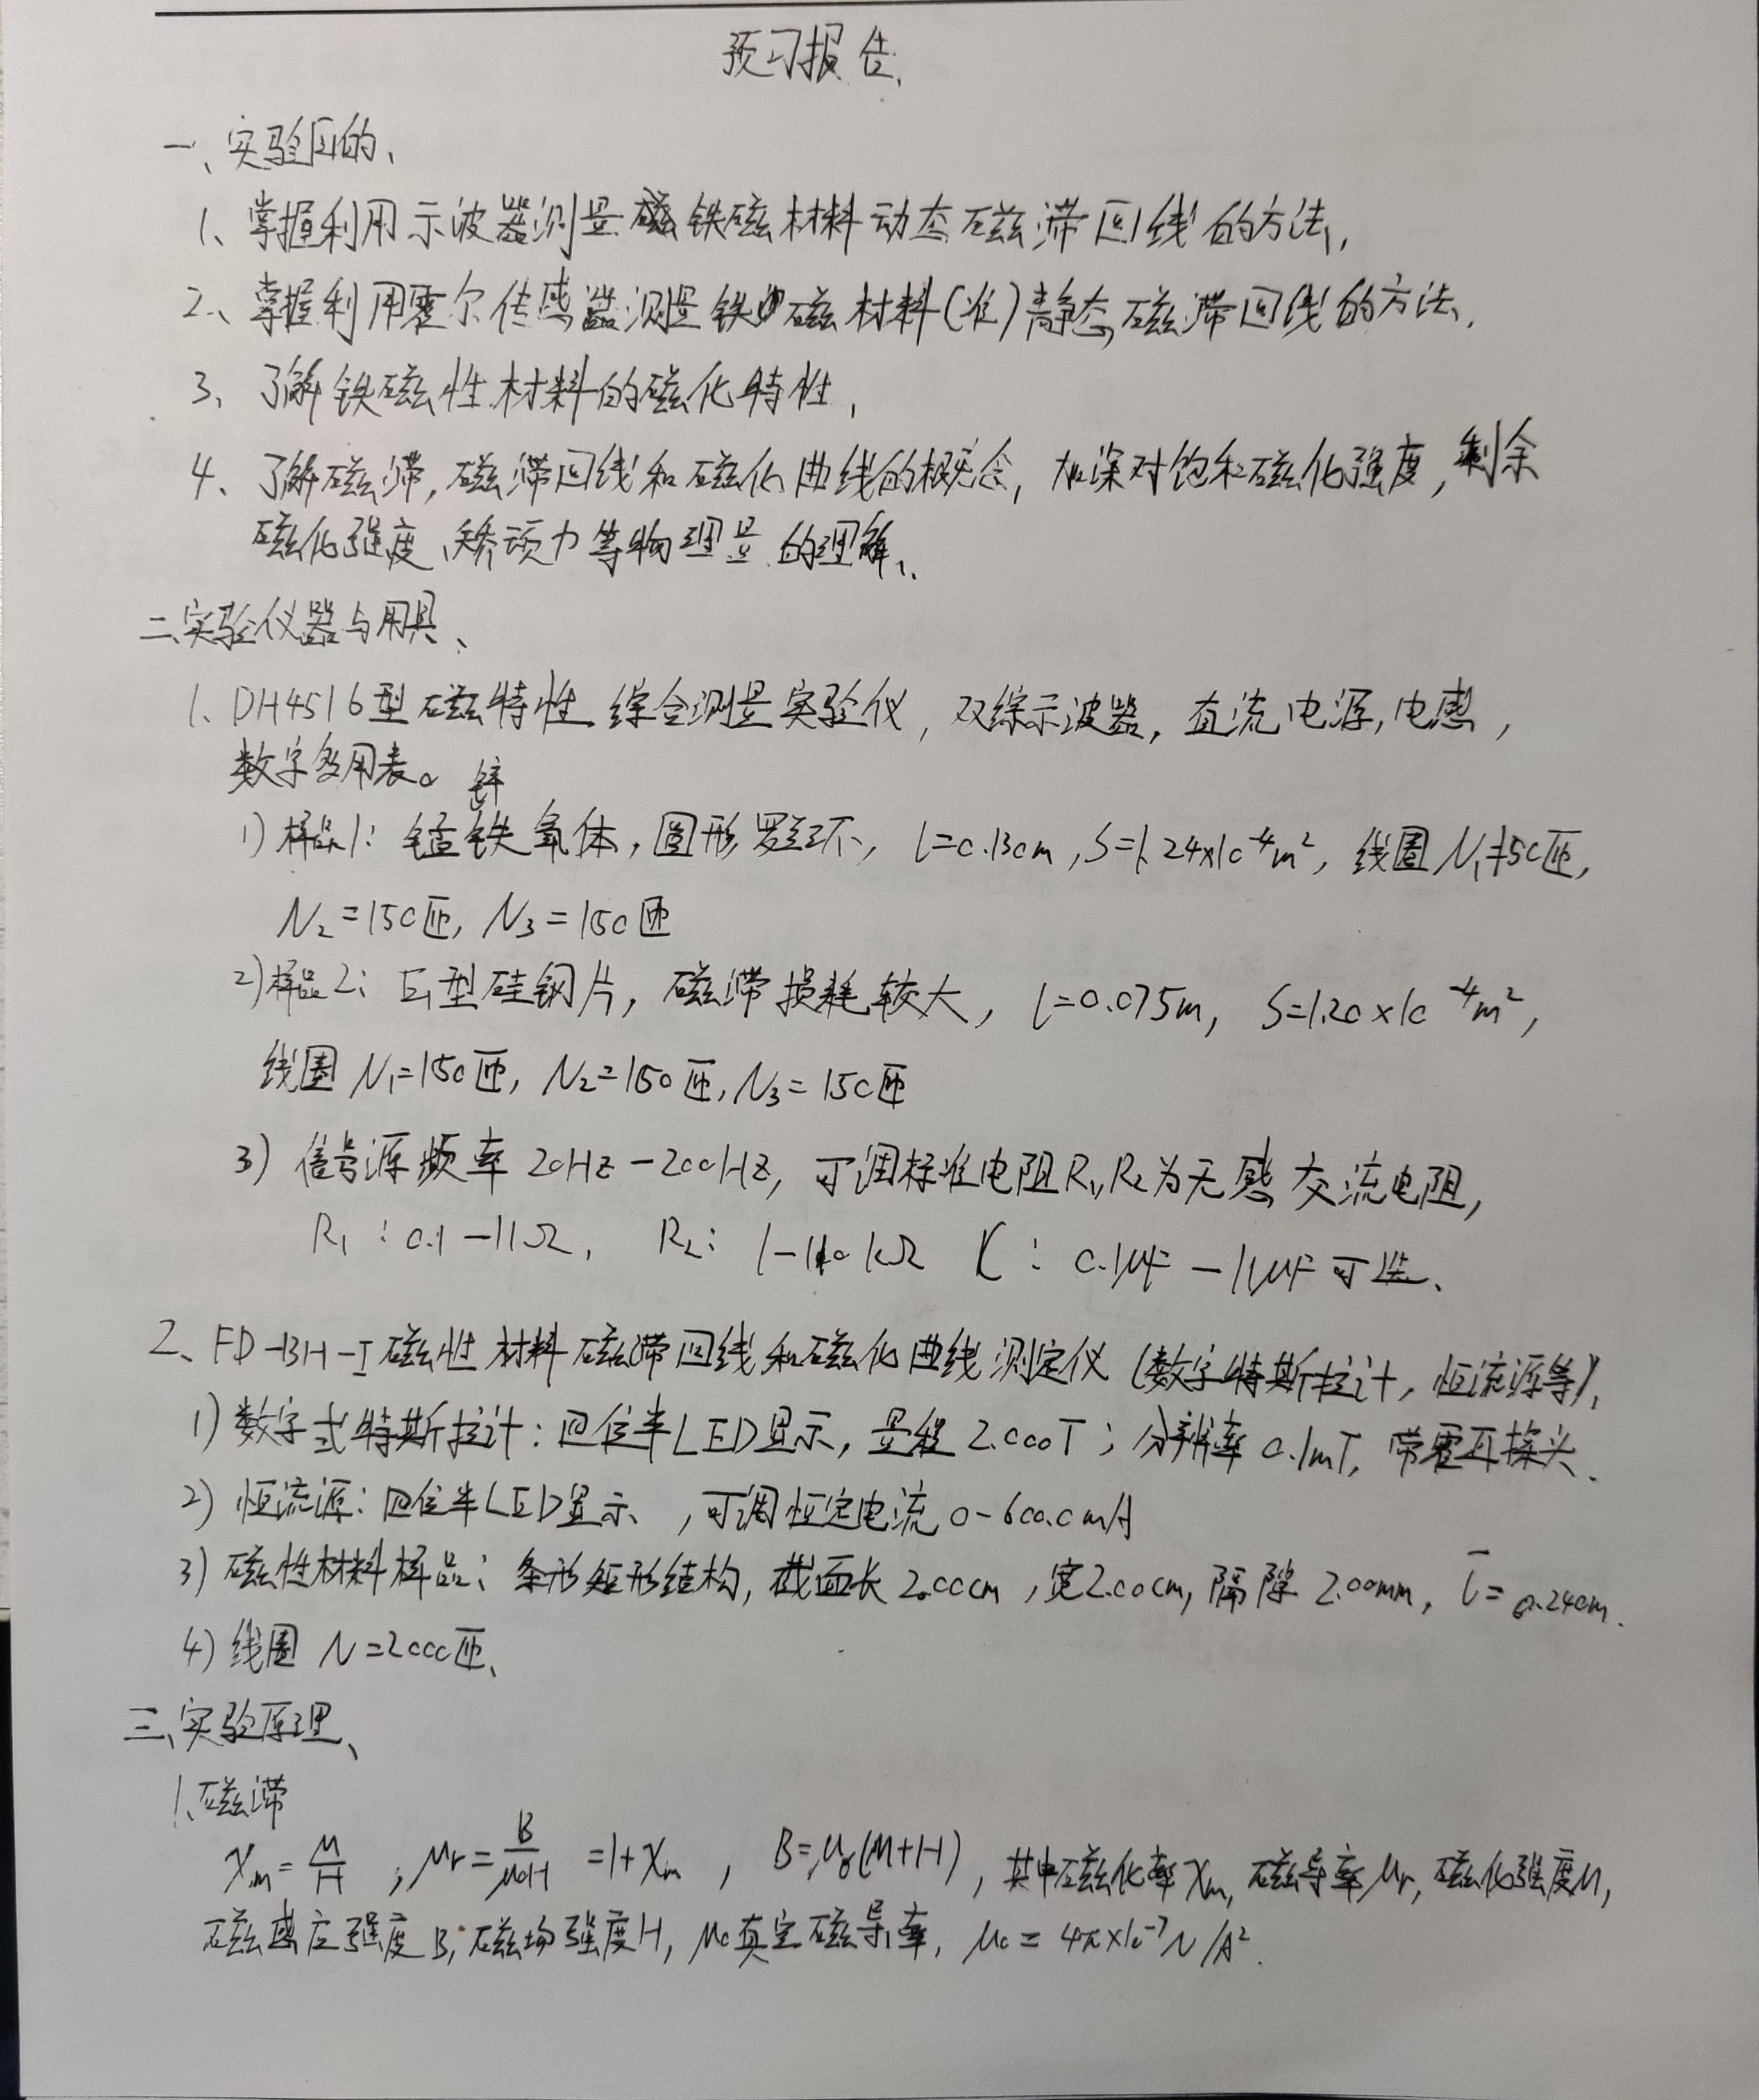
\includegraphics[width=15.5cm]{Fig/1.jpg}
        %\caption{}
    \end{figure}
    \begin{figure}[H]
        \centering
        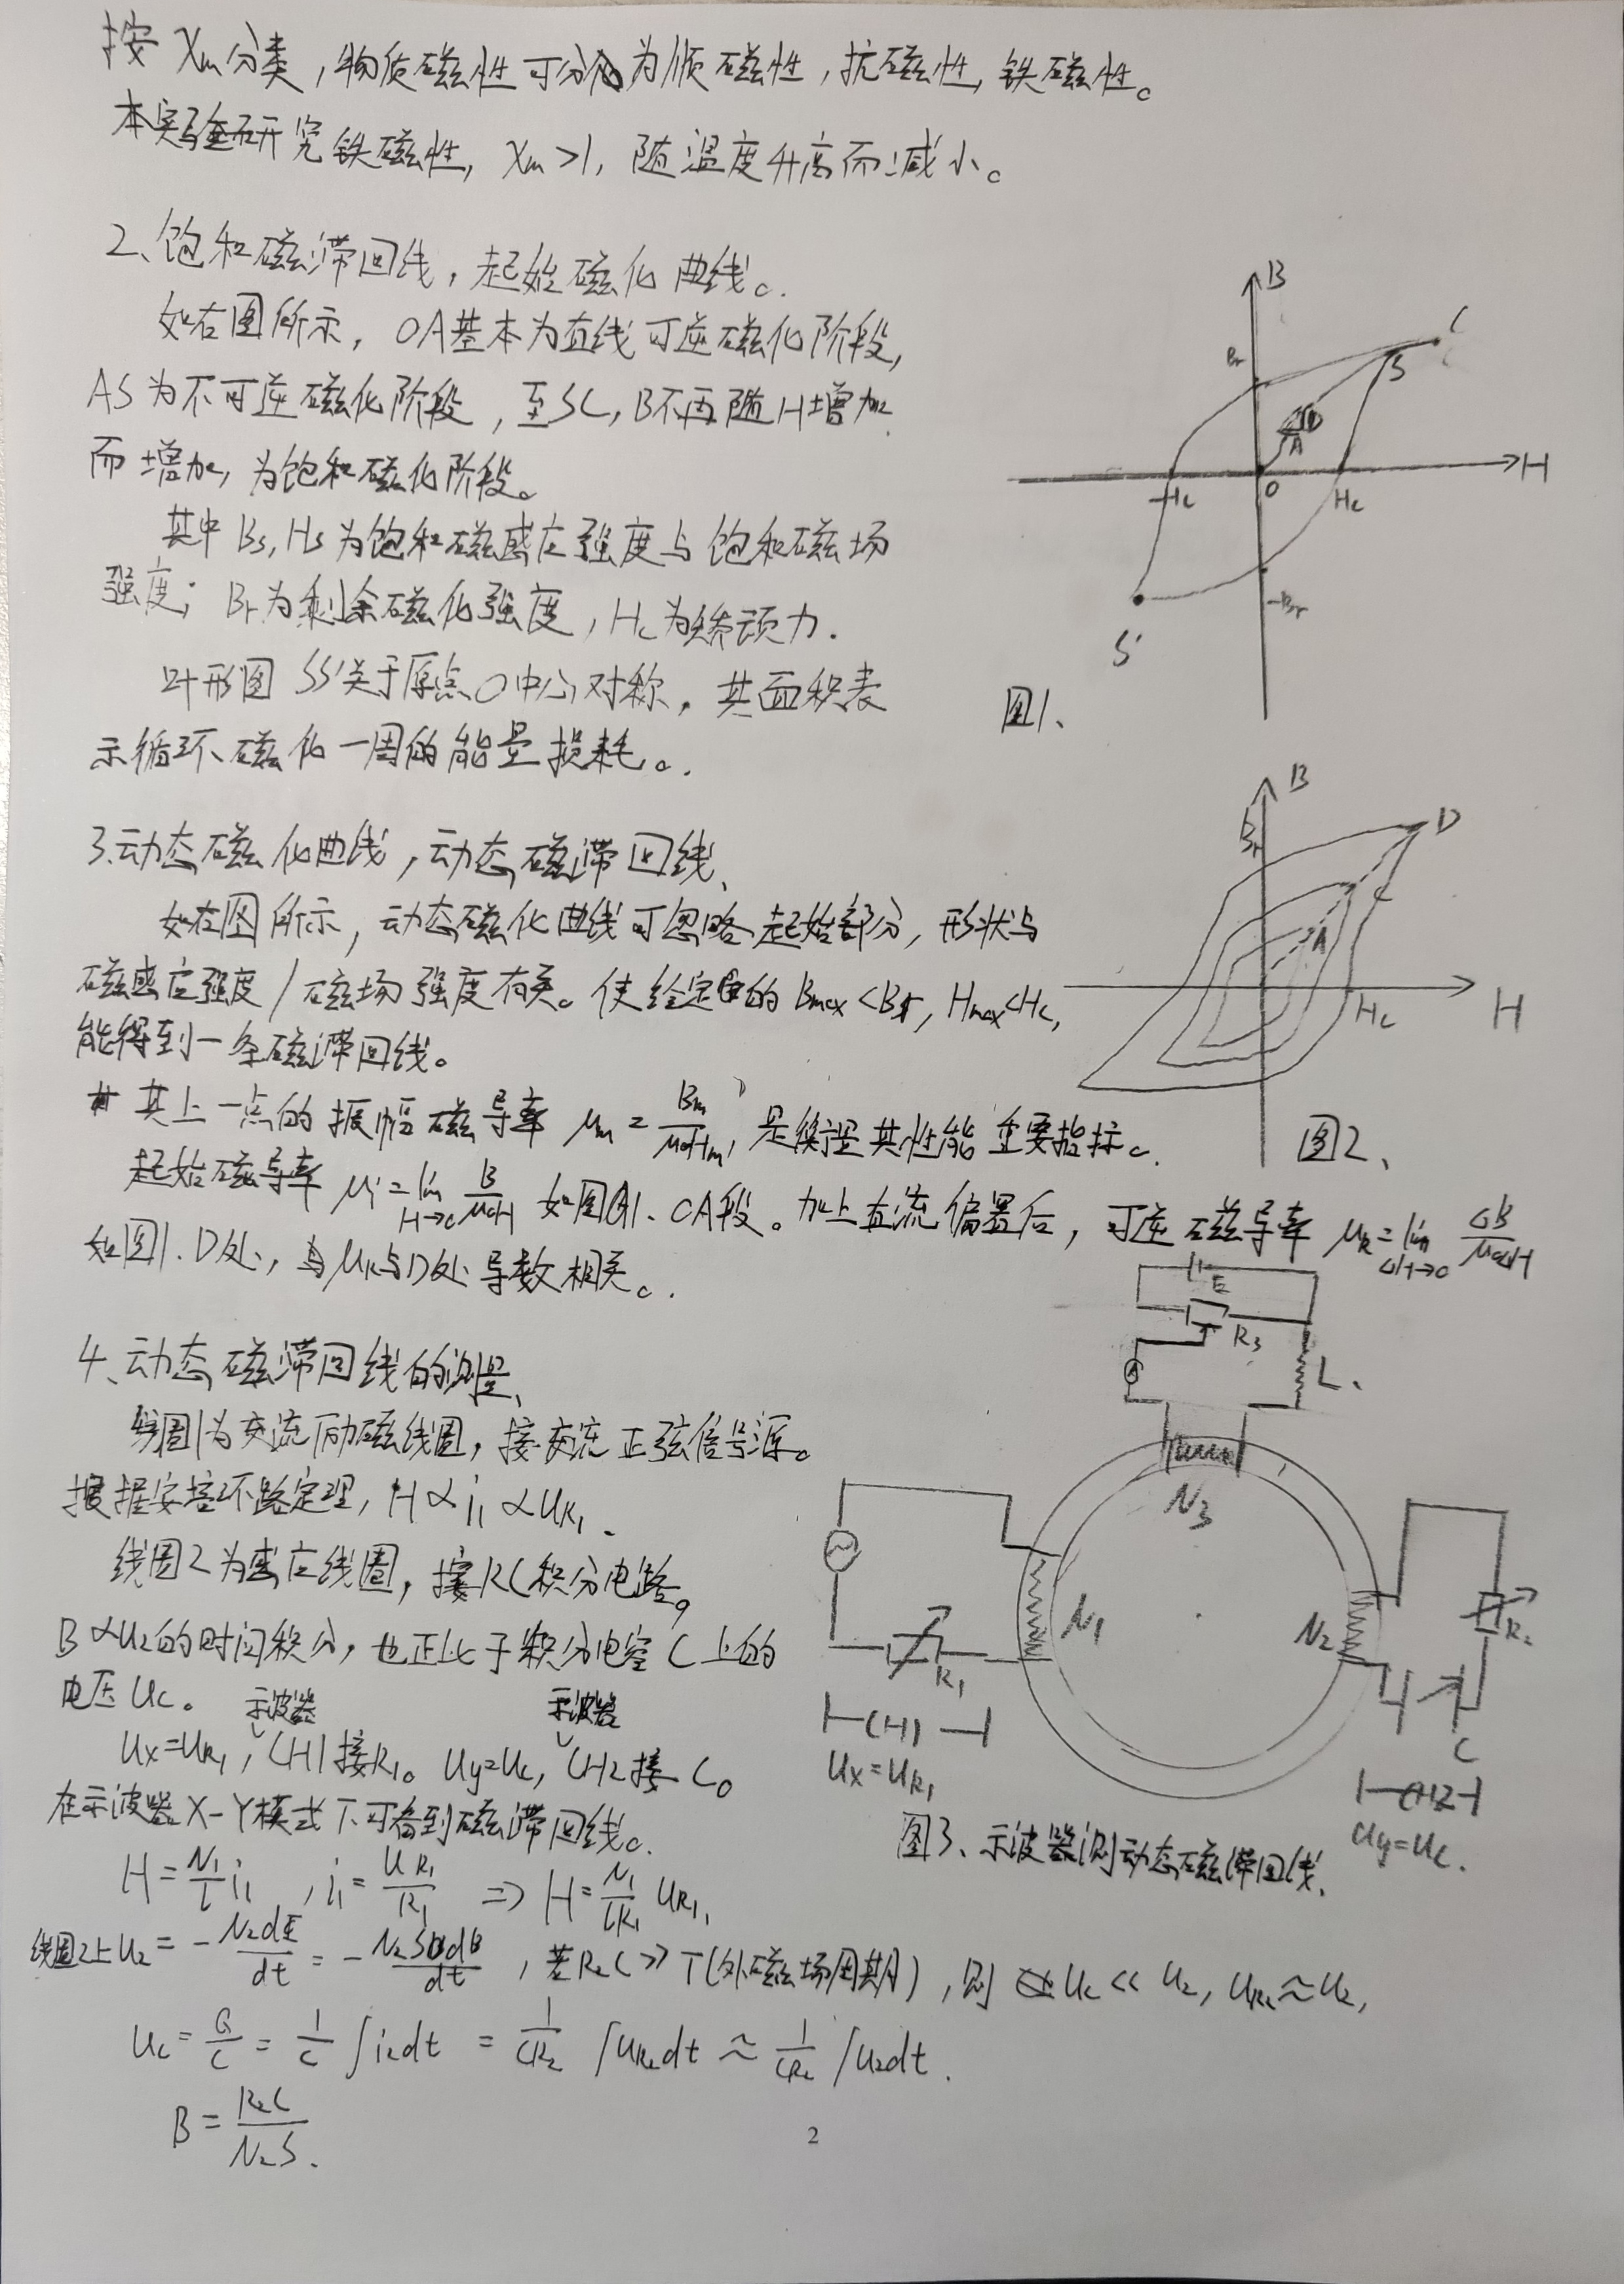
\includegraphics[width=16cm]{Fig/2.jpg}
        %\caption{}
    \end{figure}
    \begin{figure}[H]
        \centering
        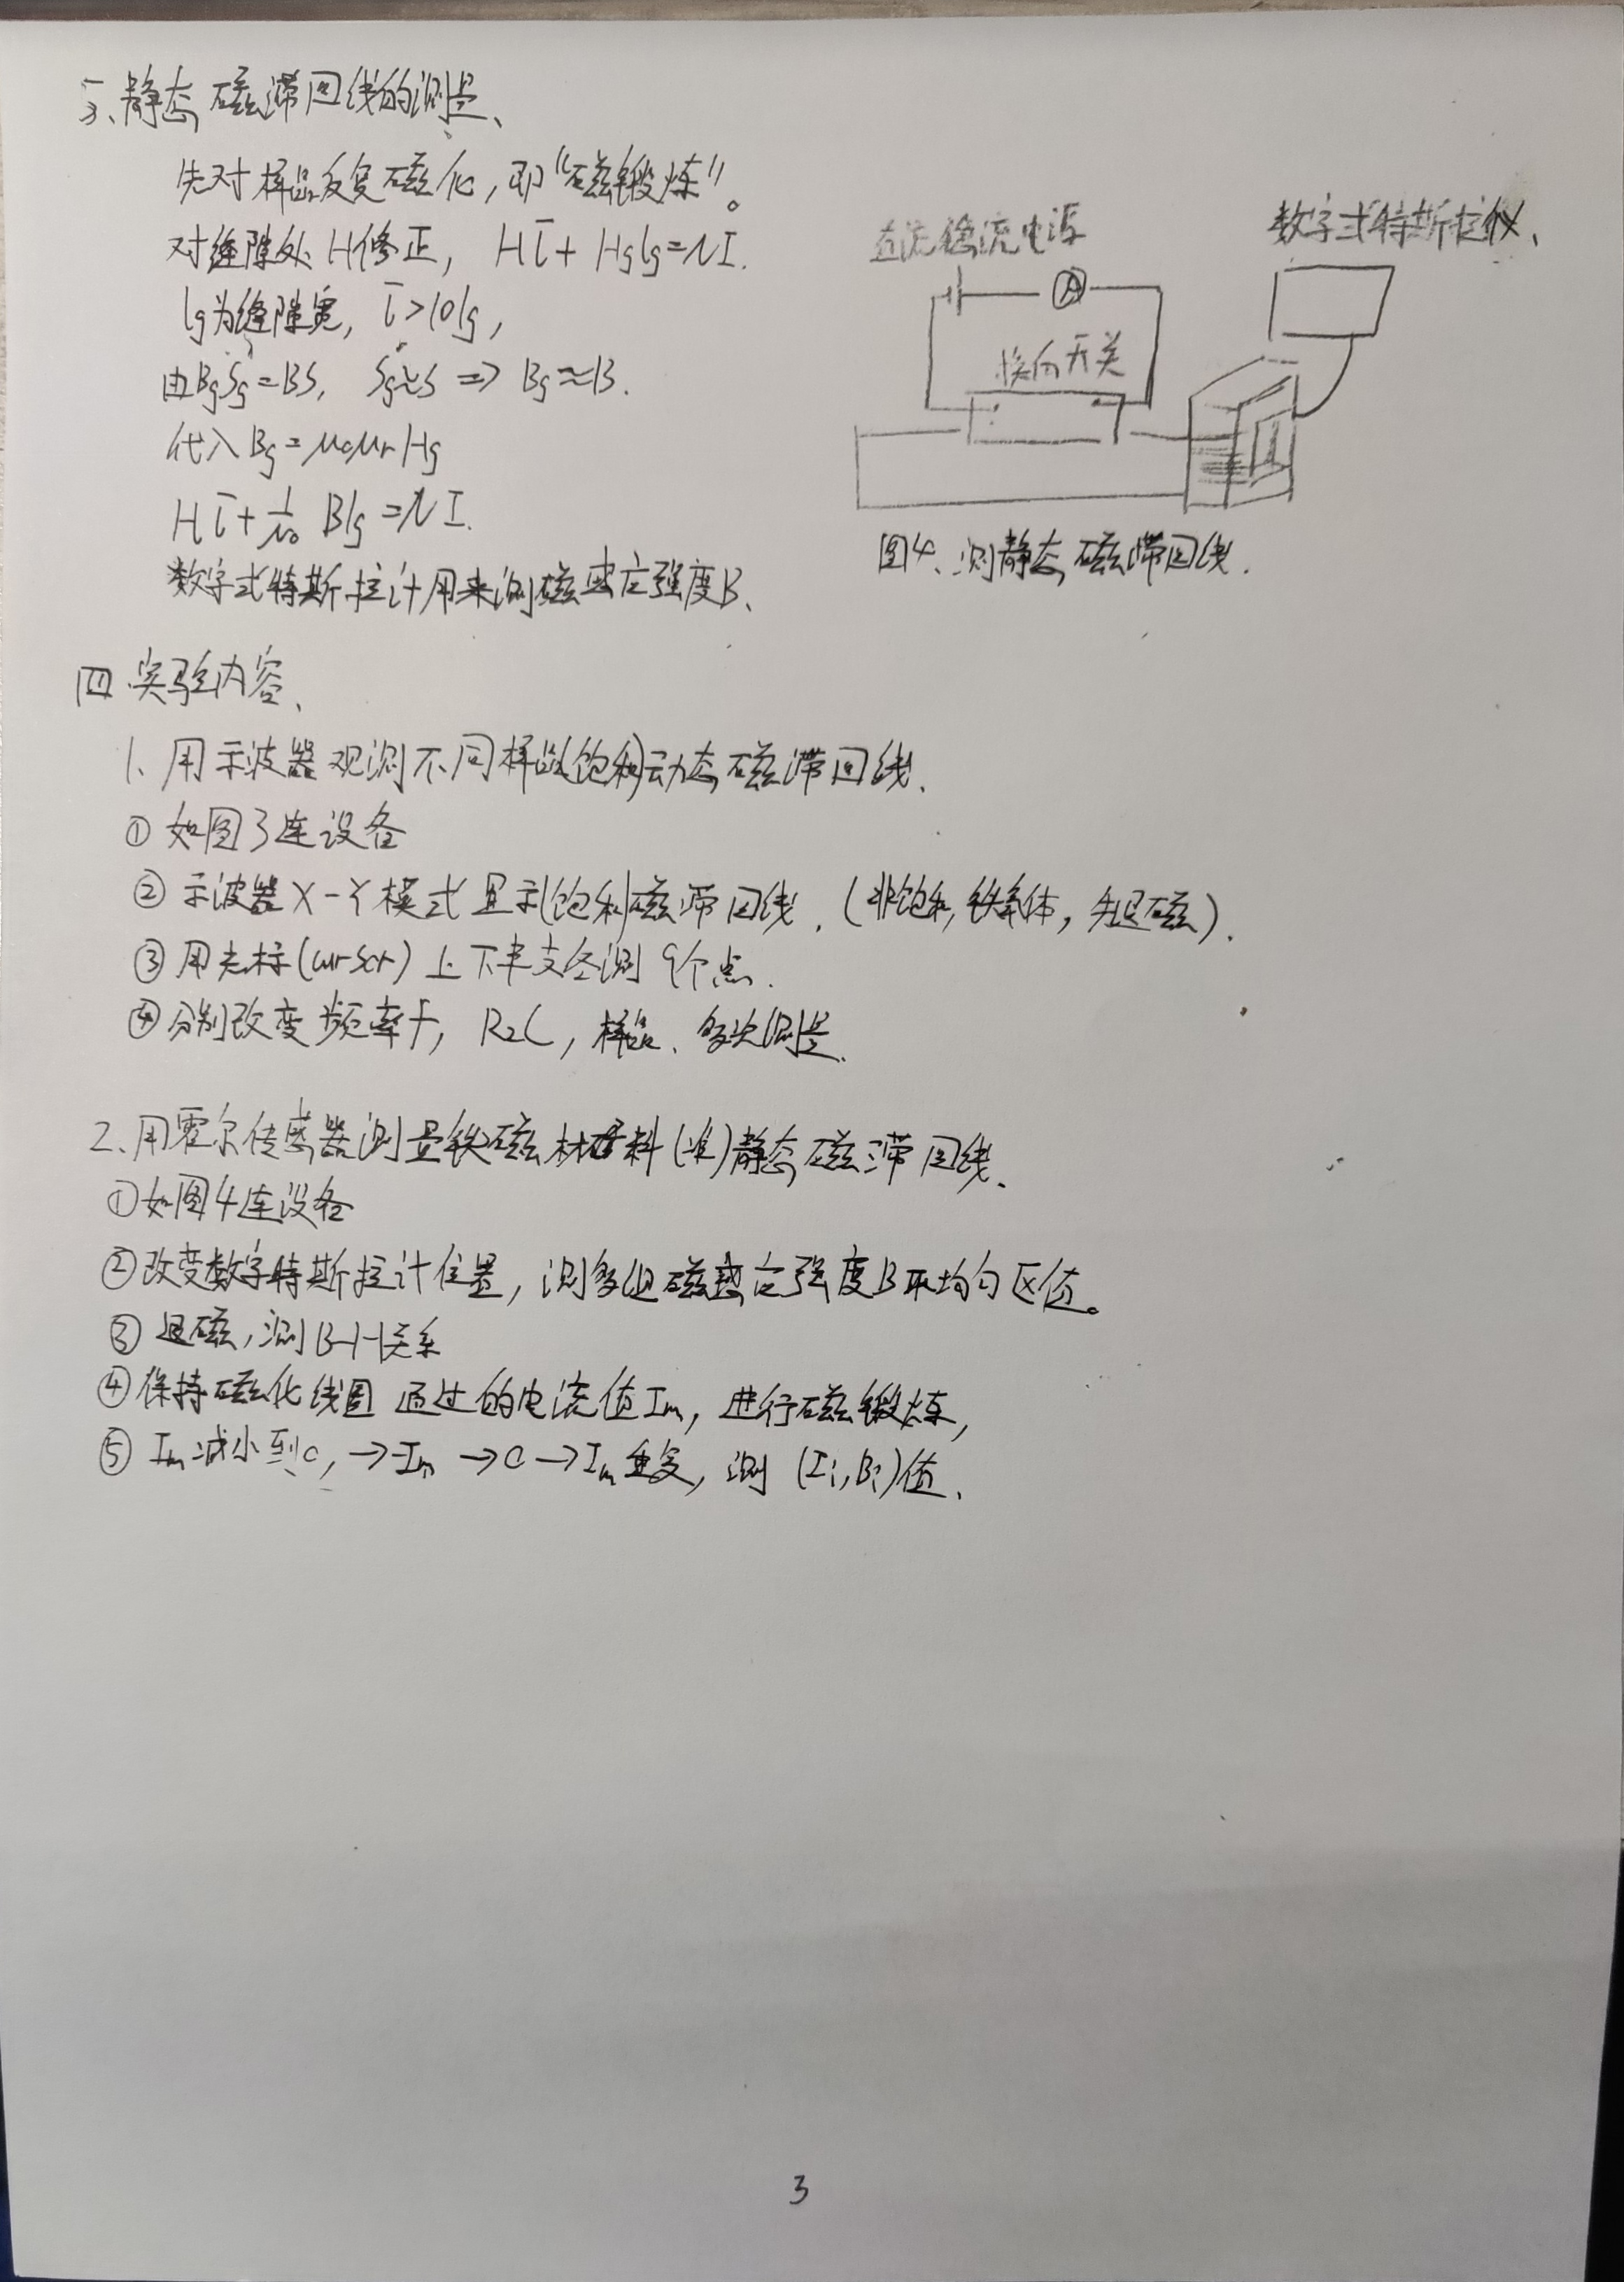
\includegraphics[width=16cm]{Fig/3.jpg}
        %\caption{}
    \end{figure}



\section{用示波器观察动态磁滞回线}
\subsection{观测样品1(铁氧体)的饱和动态磁滞回线}
\subsubsection{测量频率$f=100Hz$时的饱和磁滞回线。取$R_1=2.0\Omega$,$R_2=50k\Omega$,$C=10.0\mu F$}
\begin{enumerate}
    \item 实验步骤(本部分实验步骤相似,不再重复叙述)
    \begin{enumerate}
        \item 按预习报告中的图三连接电路,选择上述频率,电阻,电容。示波器选择X-Y模式。
        \item 调节励磁电流大小及示波器的垂直、水平位移旋钮以及振幅旋钮,在示波器显示屏上调出一个相对于坐标原点对称的饱和磁滞回线。
        \item 测量并画出饱和磁滞回线的$B-H$图。可用光标cursur测量。
    \end{enumerate}
    \item 实验数据
    \begin{enumerate}
        \item 数据计算与修正
        \newline \hspace*{2em}实验中测量$H$与$B$是按电压$u/mV$记录的。根据$H=\frac{N_1}{lR_1}u_{R_1}=577u_{R_1}$,$B=\frac{R_2C}{N_2S}u_C=26.9u_C$修正实验数据。
        \item 数据记录
        % Table generated by Excel2LaTeX from sheet 'Sheet1'
        \begin{table}[H]
          \centering
          \caption{饱和磁滞回线(竖直方向成对测量)}
            \begin{tabular}{|c|c|c|c|c|c|}\hline
            $u_{R_1}/mV$ & 点1$u_C/mV$ & 点2$u_C/mV$ & $H/H$ & 点1$B/T$ & 点2$B/T$ \\\hline
            -84    & \multicolumn{2}{|c|}{-17.4} & -48.47($-H_s$) & \multicolumn{2}{|c|}{-0.47($-B_s$)} \\\hline
            -40    & \multicolumn{1}{|c|}{-12.4} & \multicolumn{1}{|c|}{-14} & -23.08 & -0.33  & -0.38 \\\hline
            -16.8  & \multicolumn{1}{|c|}{-4.88} & \multicolumn{1}{|c|}{-9.76} & -9.69  & -0.13  & -0.26 \\\hline
            0      & \multicolumn{2}{|c|}{3.8} & 0      & \multicolumn{2}{|c|}{0.1($B_r$)} \\\hline
            15     & \multicolumn{1}{|c|}{8.8} & \multicolumn{1}{|c|}{3.2} & 8.66   & 0.24   & 0.09 \\\hline
            40     & \multicolumn{1}{|c|}{13.6} & \multicolumn{1}{|c|}{11.2} & 23.08  & 0.37   & 0.3 \\\hline
            84.4   & \multicolumn{2}{|c|}{18} & 48.7($H_s$)   & \multicolumn{2}{|c|}{0.48($B_s$)} \\\hline
            8.2    & \multicolumn{2}{|c|}{0} & 4.73($H_c$)   & \multicolumn{2}{|c|}{0}  \\\hline
            \end{tabular}%
          \label{tab:饱和磁滞回线1}%
        \end{table}%
        测量结果:$H_s=48.6A/m$,$B_s=0.475T$,$H_c=4.73A/m$,$B_r=0.1T$。查询资料得,$H_c$范围在$10 \sim 1A/m$,$\mu_0M_s=B_s-\mu_0H_s=0.5T\approx B_s$,测量结果较为合理。
                % Table generated by Excel2LaTeX from sheet 'Sheet1'
        \begin{table}[H]
          \centering
          \caption{饱和磁滞回线(水平方向成对测量)}
            \begin{tabular}{|c|c|c|c|c|c|}\hline
            $u_C/mV$   & 点1$u_{R_1}/mV$ & 点2$u_{R_1}/mV$     & $B/T$  & 点1$H/H$    & 点1$H/H$ \\\hline
            -7.76  & -24    & -11    & -0.21  & -13.85 & -6.35 \\\hline
            -4     & -15.8  & -1     & -0.11  & -9.12  & -0.58 \\\hline
            0      & -8.2   & 8.2    & 0      & -4.73  & 4.73 \\\hline
            4.8    & 3      & 17.8   & 0.13   & 1.73   & 10.27 \\\hline
            9.4    & 17     & 28.4   & 0.25   & 9.81   & 16.39 \\\hline
            \end{tabular}%
          \label{tab:饱和磁滞回线2}%
        \end{table}%
        (注:$H_s$,$H_r$,$B_s$,$B_r$只测量一次,在水平方向测量时不再次测量。)
        \begin{figure}[H]
            \centering
            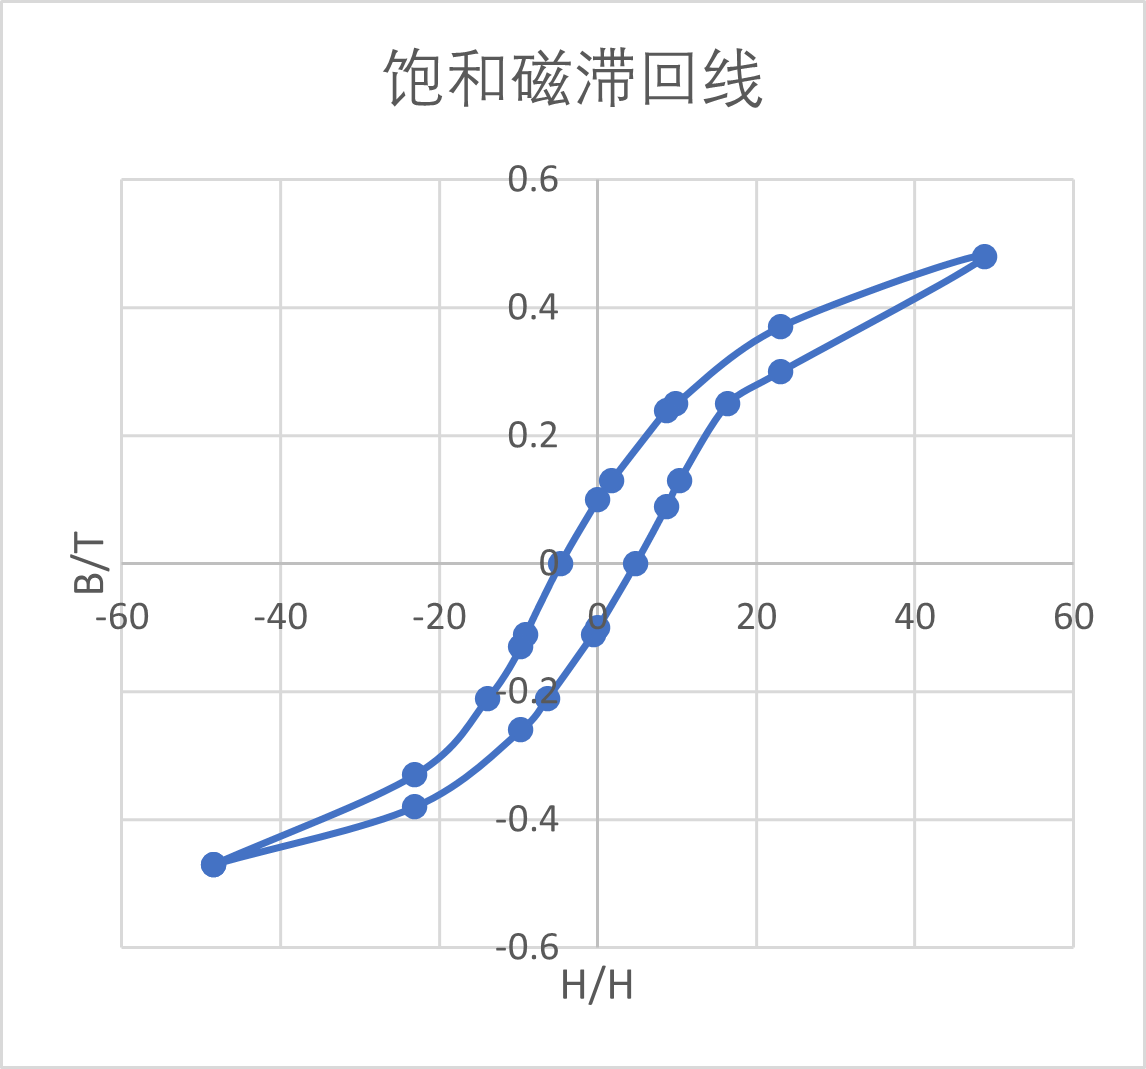
\includegraphics[width=8cm]{Fig/4.png}
            \caption{动态磁滞回线}
        \end{figure}
        可以看到,数据点形成的平滑曲线近似为磁滞回线。由于测量点较少,不足20个,磁滞回线光滑度较差。并且从趋势上,可能未饱和磁化,会带来测量误差。实际上,恰好饱和磁化的曲线难以肉眼判断。

    \end{enumerate}
\end{enumerate}

\subsubsection{固定信号源幅度,观测并记录饱和磁滞回线随频率的变化规律}
\begin{enumerate}
    \item 保持$R_1$,$R_2C$不变,测量并比较$f=95Hz$和$f=150Hz$时的$B_r$和$H_c$。
    \begin{table}[H]
        \centering
        \caption{不同频率下$B_r/T$和$H_c/H$}
          \begin{tabular}{|c|c|c|}\hline
                & $95Hz$  &  $150Hz$\\\hline
            $B_r/T$ & 0.108     & 0.070 \\\hline
            $H_c/H$ & 4.73    & 4.73 \\\hline
          \end{tabular}%
        \label{tab:tab3}%
    \end{table}%
    \hspace*{2em}可以看到,$B_r$随频率增大而减小,$H_c$不变。$H_c$是矫顽力,为材料的特性。
    电路中,励磁线圈存在电感。频率越高,励磁线圈的自感电动势越大,导致磁场测量部分的分压减小。因此$B_r$呈减小趋势。
    \item 在频率$f=50Hz$下,比较不同积分常量取值对李萨如图的影响。
    \newline \hspace*{2em}固定励磁电流幅度$I_m=0.1A$,$R_1=2.0\Omega$。
    \begin{figure}[H]
        \centering
        \begin{minipage}[t]{0.33\linewidth}
            \centering
            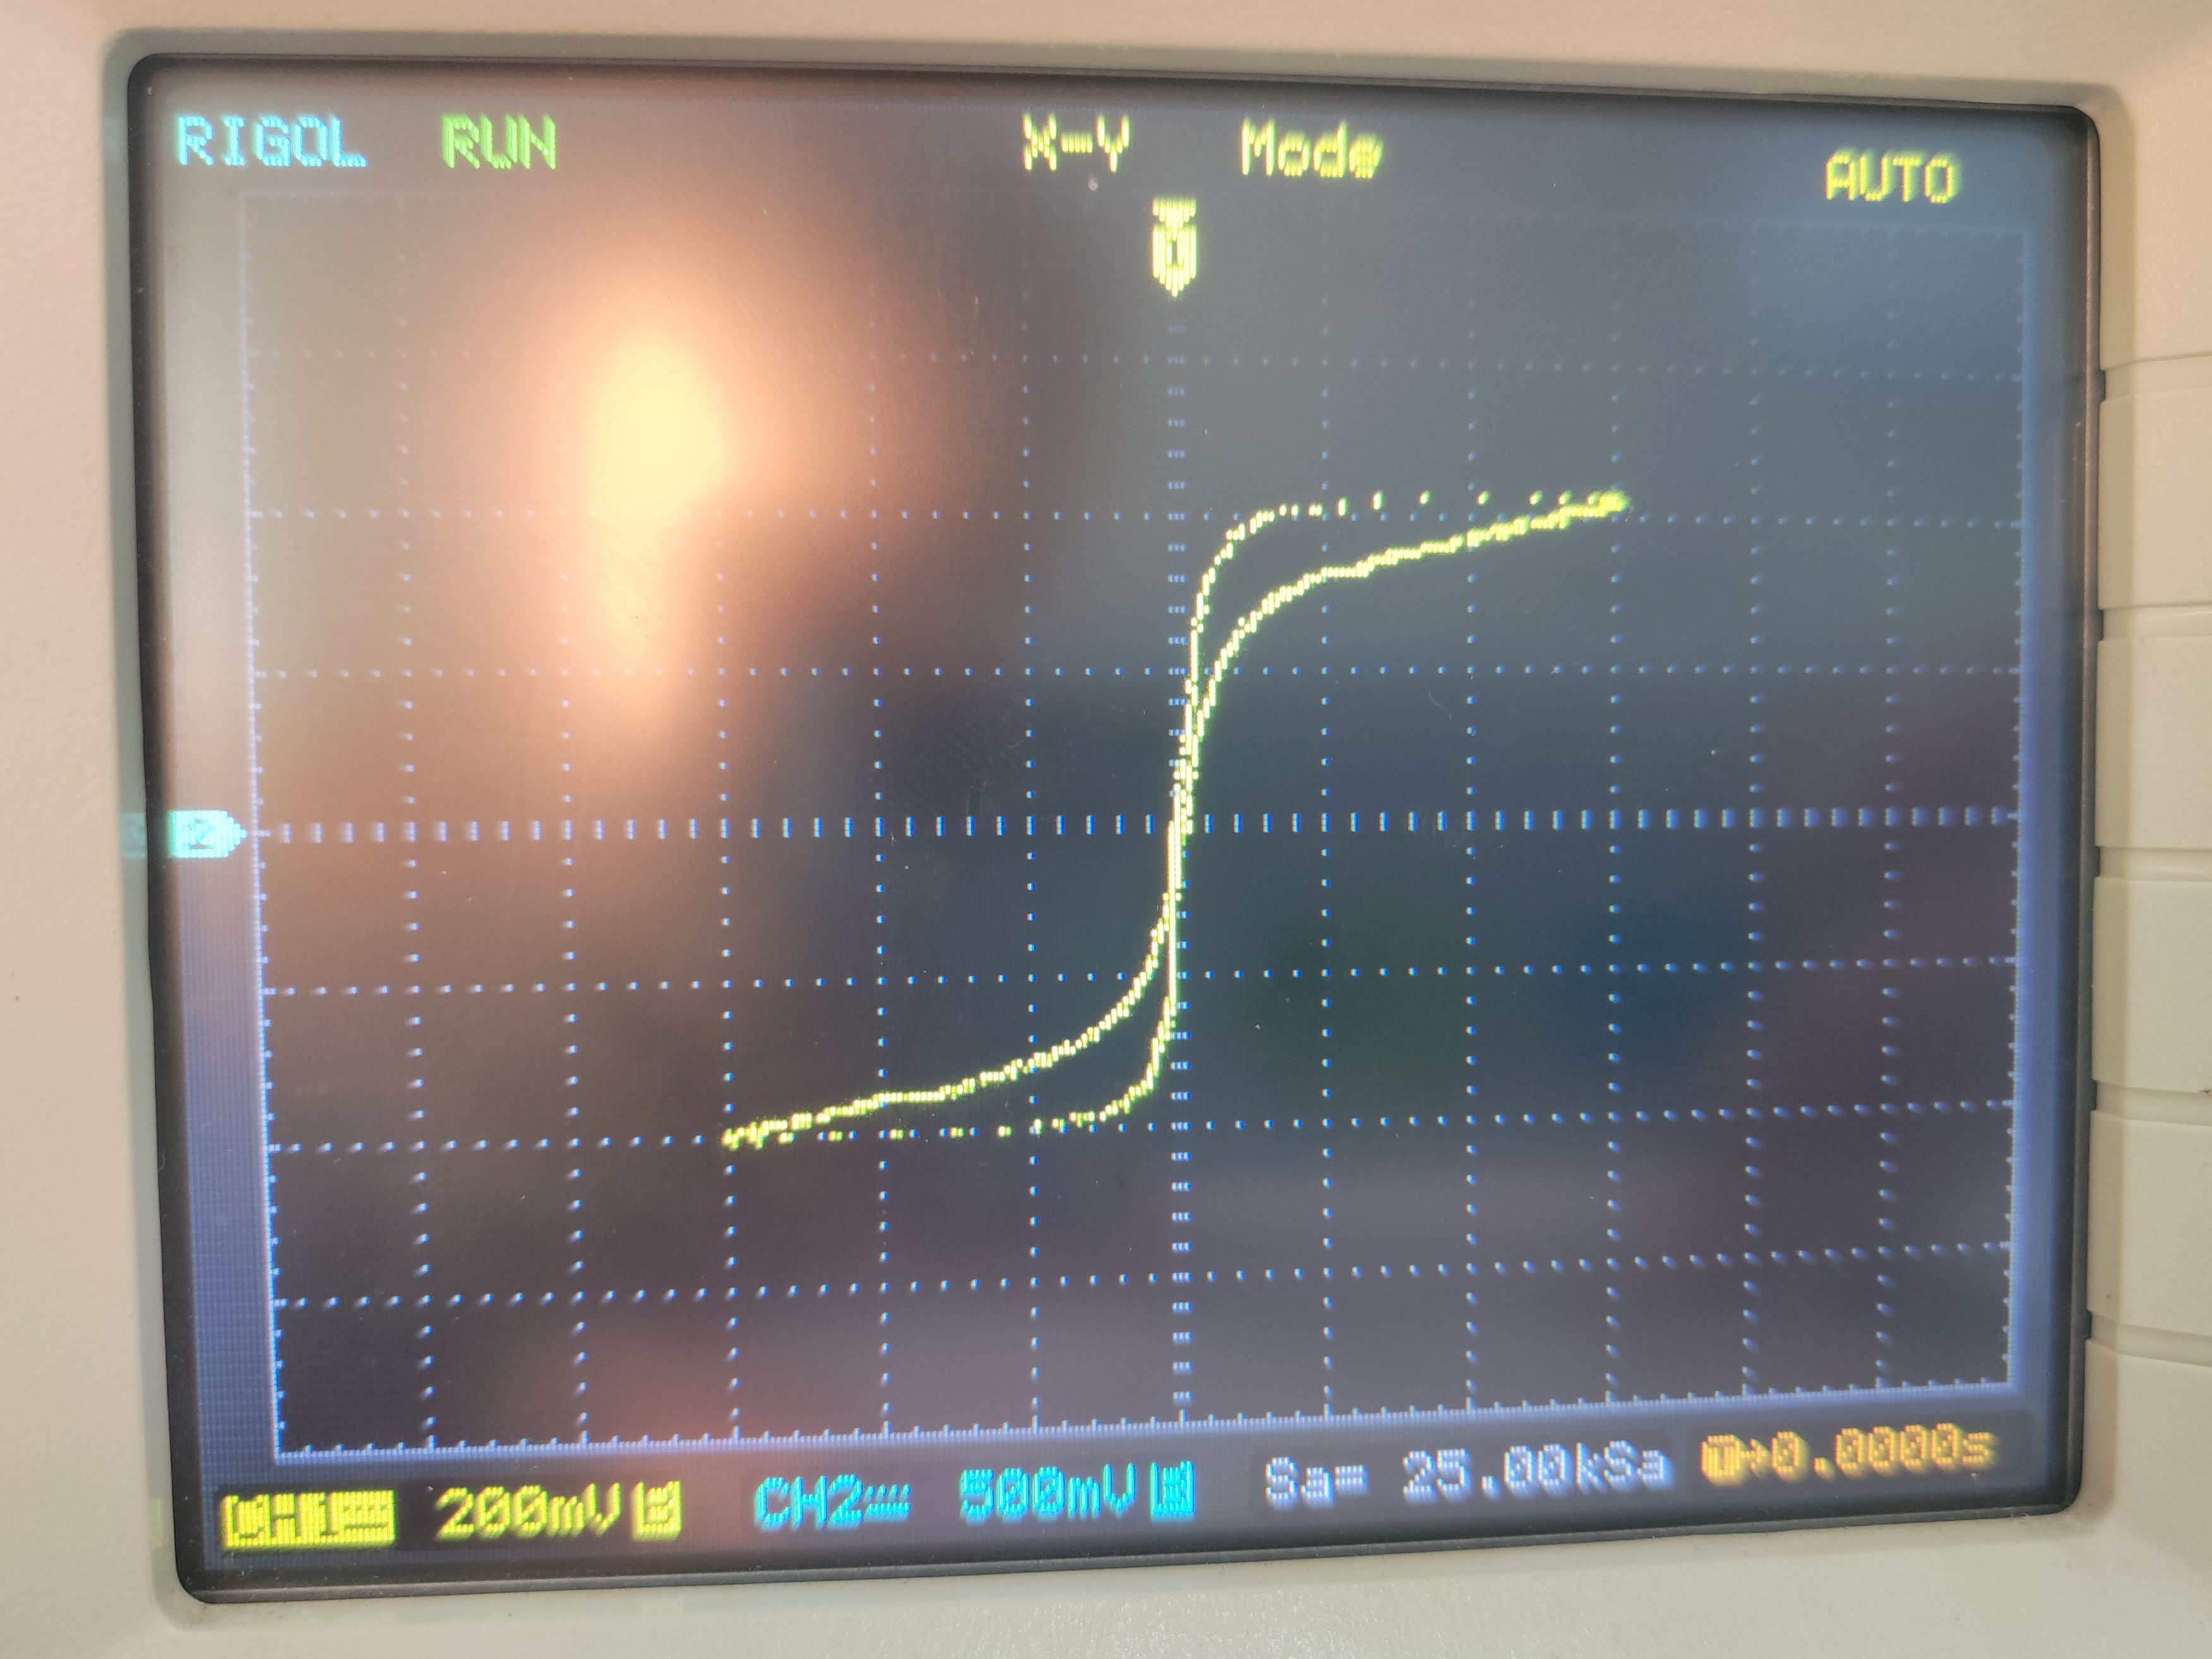
\includegraphics[width=5.2cm]{Fig/5-0.01.jpg}
            \caption{$R_2C=0.01s$}
        \end{minipage}
        \begin{minipage}[t]{0.33\linewidth}
            \centering
            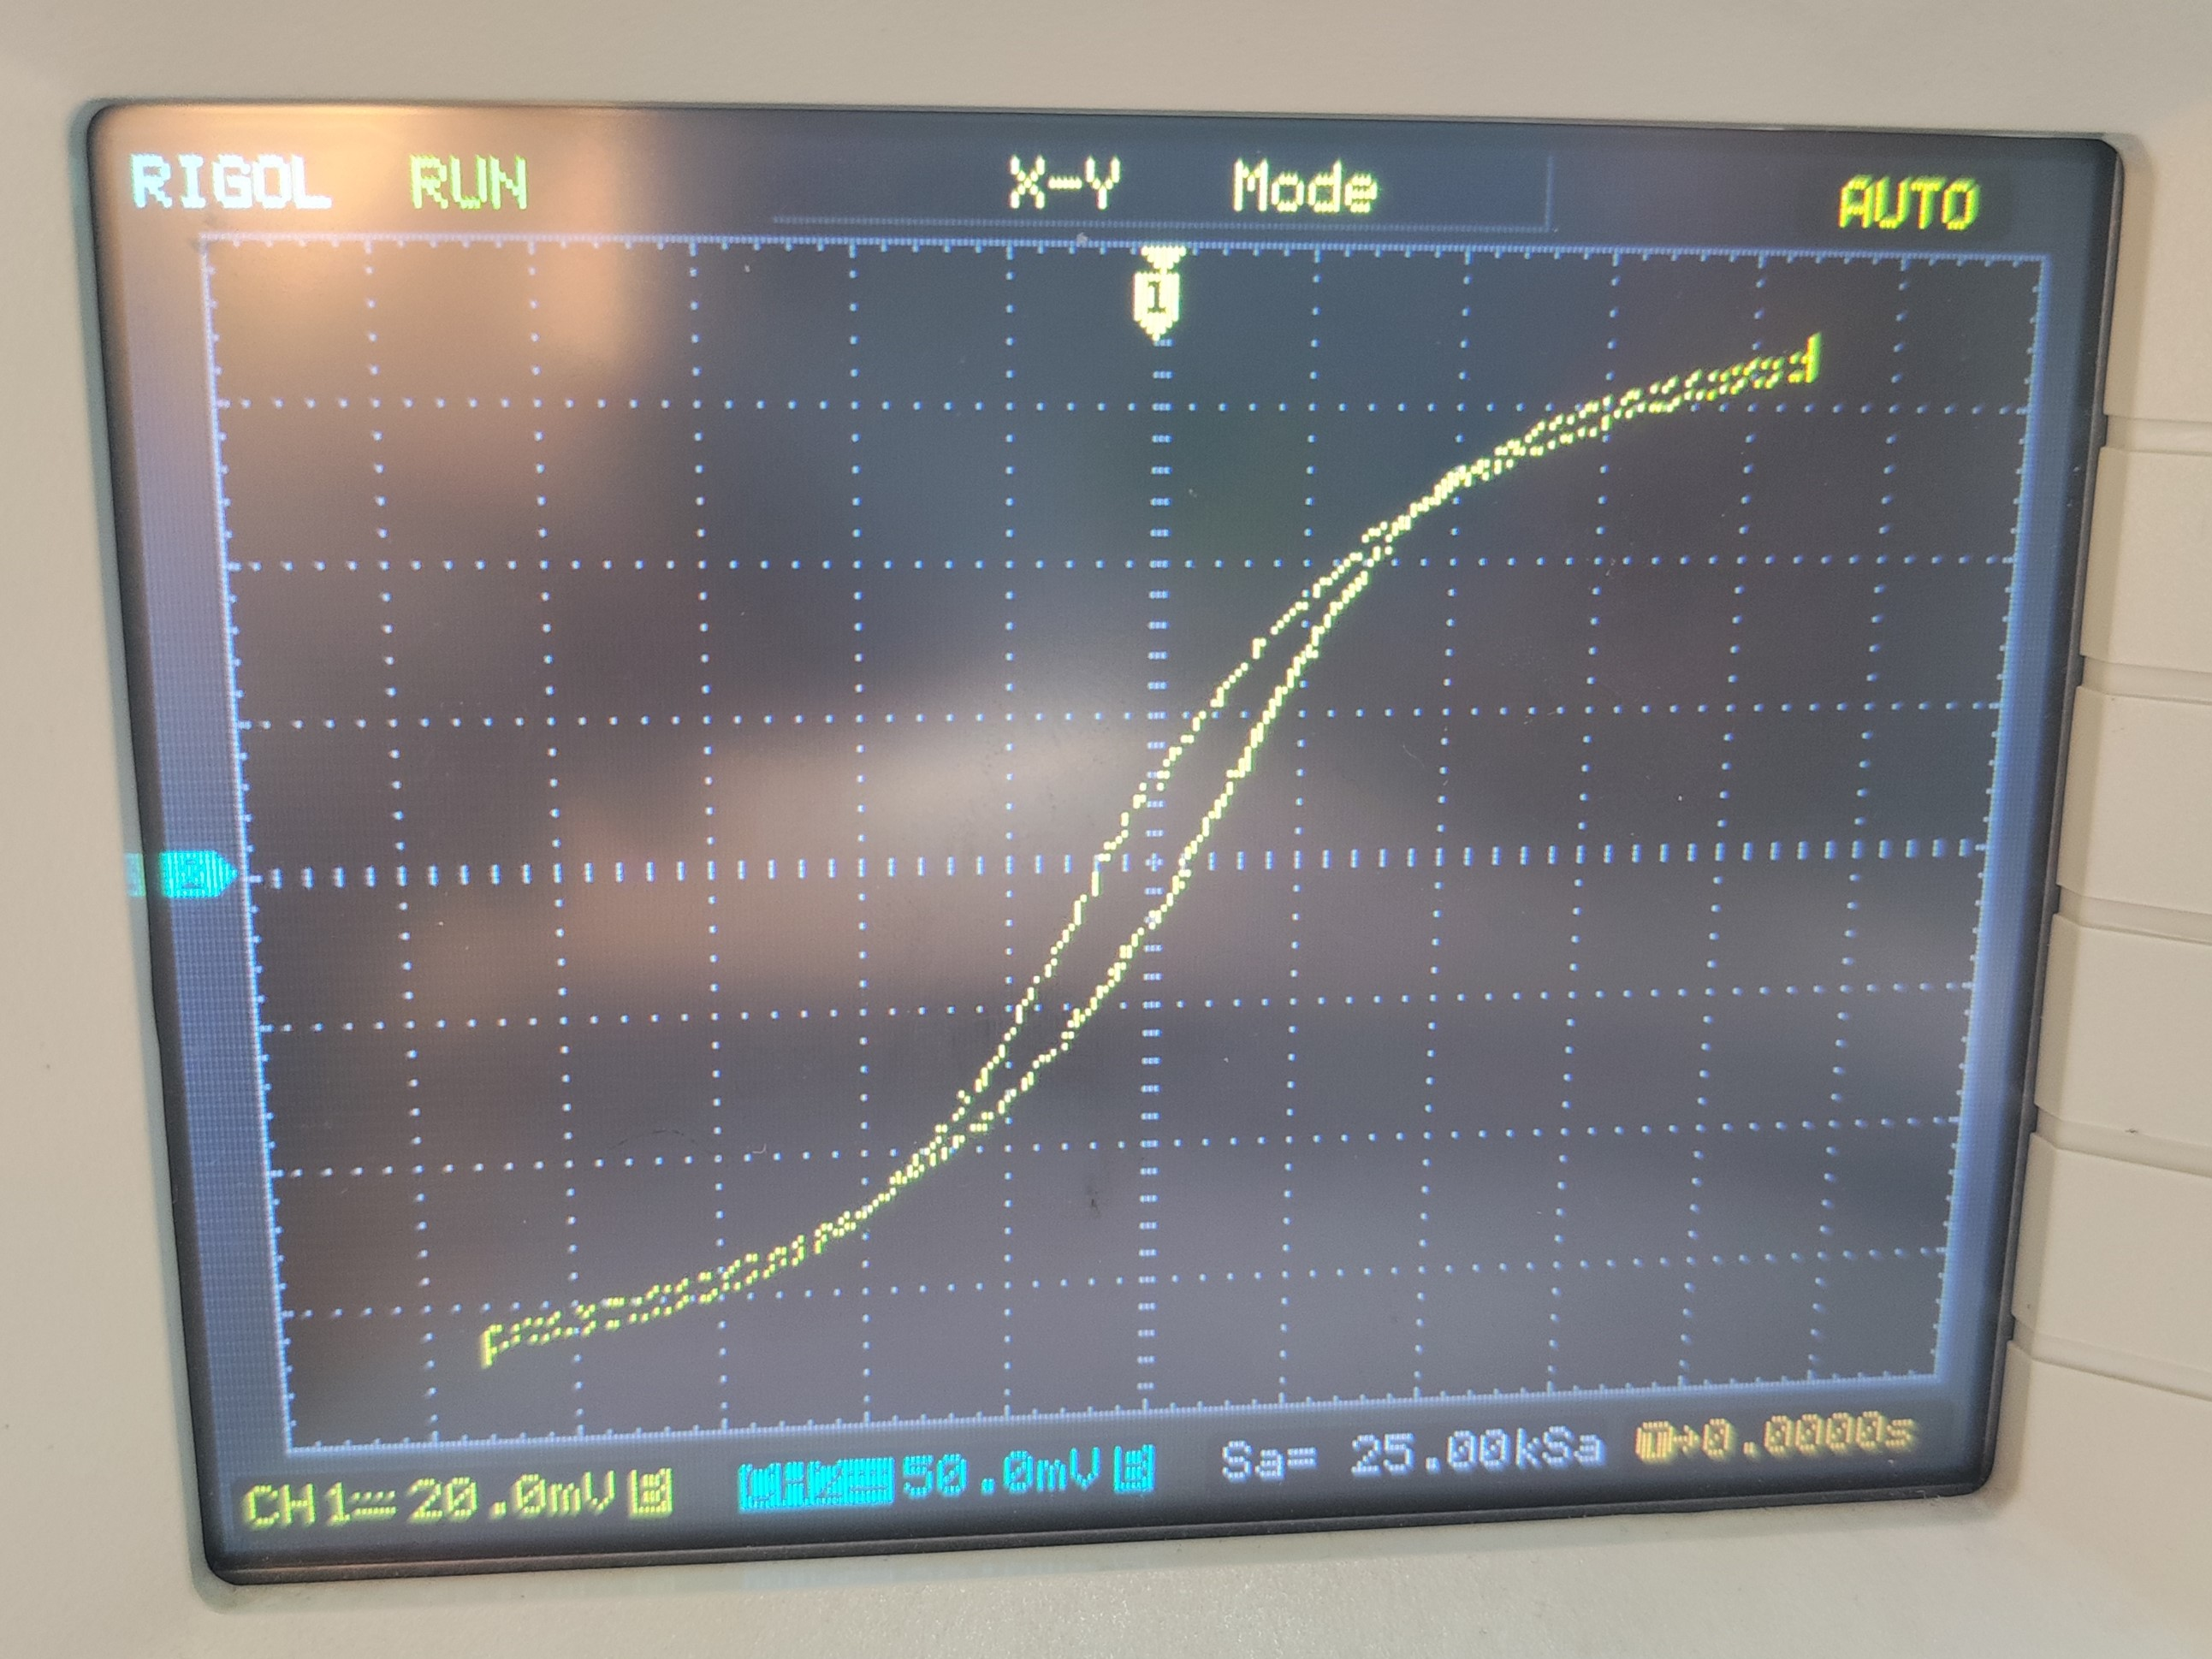
\includegraphics[width=5.2cm]{Fig/5-0.05.jpg}
            \caption{$R_2C=0.05s$}
        \end{minipage}
        \begin{minipage}[t]{0.33\linewidth}
            \centering
            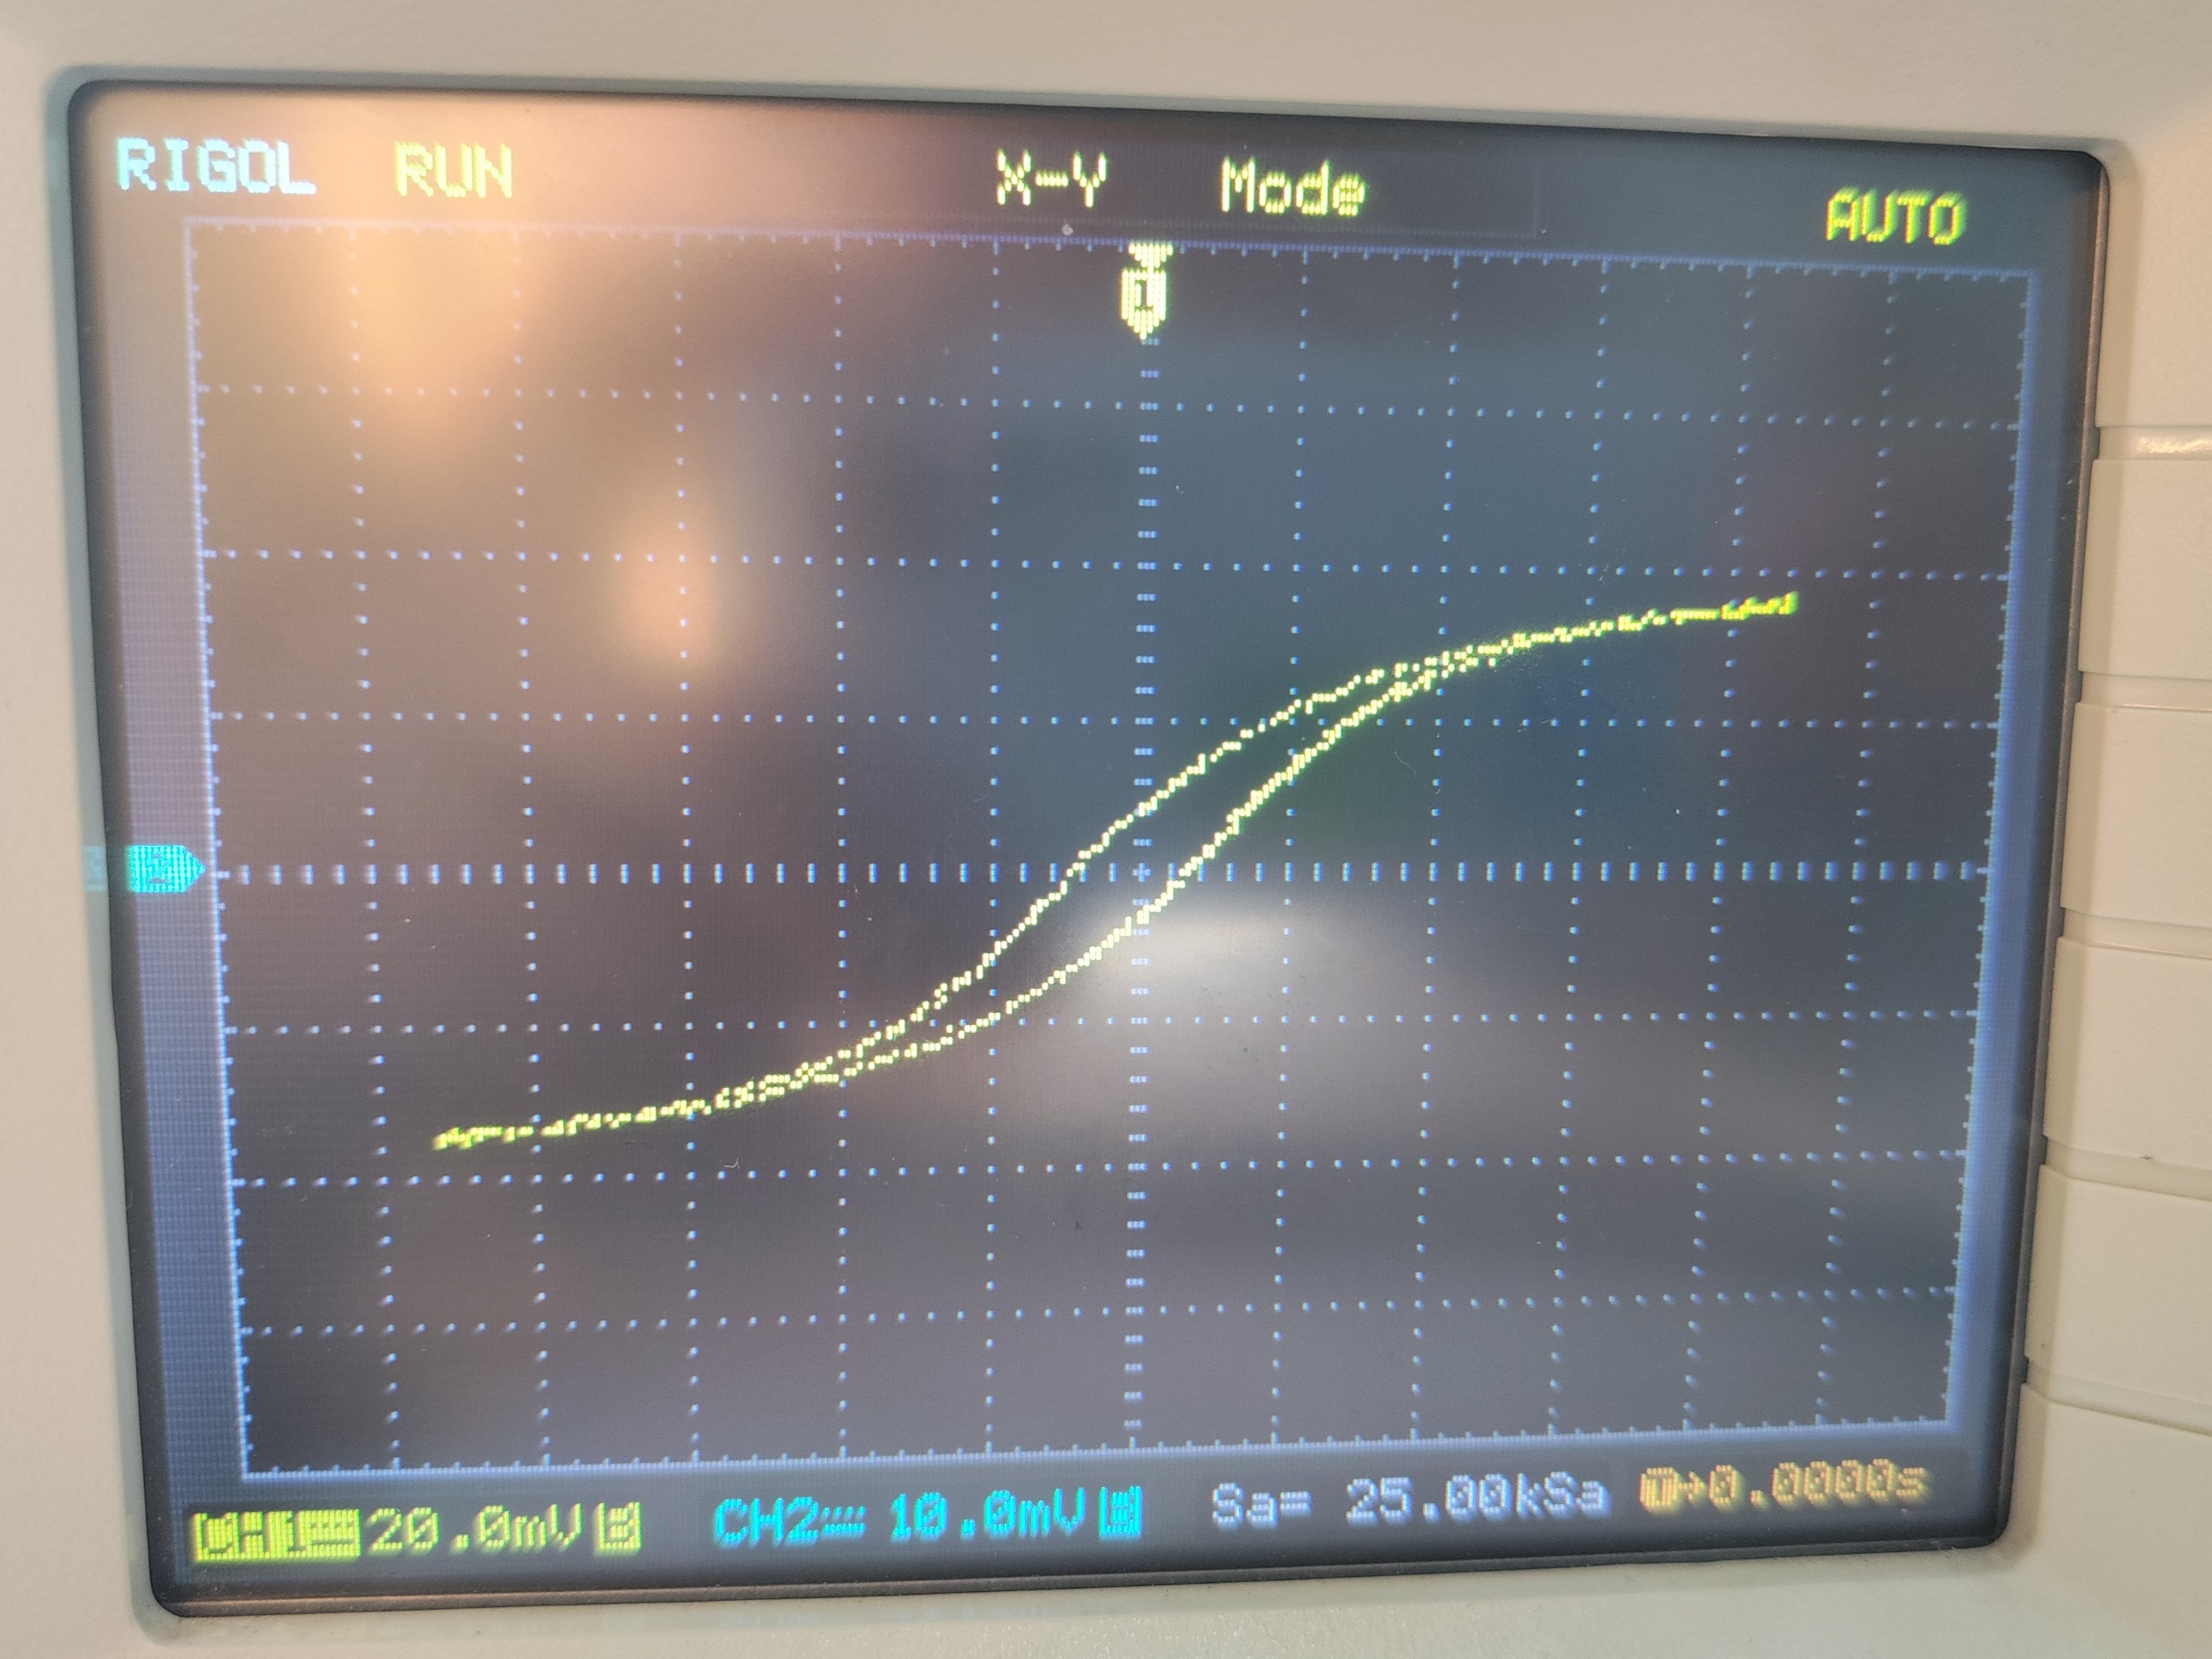
\includegraphics[width=5.2cm]{Fig/5-0.5.jpg}
            \caption{$R_2C=0.5s$}
        \end{minipage}
        
    \end{figure}
    (1)积分常量为什么影响李萨如图像的形状?
    \newline 由公式
    \[u_C=\frac{Q}{C}=\frac{1}{C}\int i_2dt=\frac{1}{CR_2}\int u_{R2}dt\approx \frac{1}{CR_2}\int u_{2}dt\]
    \hspace*{2em}公式推导时,约等于要求积分常量$R_2C\gg T$,此时$u_{R2}\approx u_2$。前面实验$f=100Hz$,$T=0.02s$,积分常量$R_2C=0.5s$,满足条件。当积分常量$R_2C=0.05s,0.01s$时,不再满足该条件,李萨如图像发生变化。
    \newline (2)积分常量是否会影响真实的磁滞回线的形状?
    \newline \hspace*{2em}由$B=\frac{R_2C}{N_2S}u_C$,$u_C$的改变会影响B的测量值,但不改变其实际值。B测量值改变导致李萨如图像变化。对$u_C$进行修正后,我们还可以得到正常的磁滞回线图像。积分常量不影响真实的磁滞回线的形状。
\end{enumerate}
\subsection{测量样品1(铁氧体)的动态磁滞回线}
\begin{enumerate}
    \item $f=100Hz$, $R_1=2.0\Omega$, $R_2=50k\Omega$, $C=10.0\mu F$。
    \item 实验中测量$H$与$B$是按电压$u/mV$记录的。根据$H=\frac{N_1}{lR_1}u_{R_1}=577u_{R_1}$,$B=\frac{R_2C}{N_2S}u_C=26.9u_C$修正实验数据。
    \item 由$\mu_m=\frac{B_m}{\mu_0 H_m}$计算$\mu_m$。
            % Table generated by Excel2LaTeX from sheet 'Sheet1'
        \begin{table}[H]
          \centering
          \caption{样品1动态磁化曲线数值}
            \begin{tabular}{|c|c|c|c|c|}\hline
            $u_{R1}/mV$    & $u_C/mV$     & $H_m/H$     & $B_m/T$     & $\mu_m/(T\cdot H^{-1})$ \\\hline
                   &        & 0      & 0      &  \\\hline
            6.4    & 2.24   & 3.6928 & 0.060256 & 12984.78 \\\hline
            8      & 2.72   & 4.616  & 0.073168 & 12613.79 \\\hline
            10     & 3.36   & 5.77   & 0.090384 & 12465.39 \\\hline
            12.8   & 4.4    & 7.3856 & 0.11836 & 12752.91 \\\hline
            15.8   & 5.28   & 9.1166 & 0.142032 & 12397.77 \\\hline
            17.8   & 6.08   & 10.2706 & 0.163552 & 12672.15 \\\hline
            20     & 6.88   & 11.54  & 0.185072 & 12762.19 \\\hline
            21.6   & 7.44   & 12.4632 & 0.200136 & 12778.67 \\\hline
            23.4   & 8.08   & 13.5018 & 0.217352 & 12810.38 \\\hline
            25.2   & 8.88   & 14.5404 & 0.238872 & 13073.11 \\\hline
            32.4   & 11.2   & 18.6948 & 0.30128 & 12824.48 \\\hline
            37.8   & 12.4   & 21.8106 & 0.33356 & 12170.17 \\\hline
            41     & 13.2   & 23.657 & 0.35508 & 11944.19 \\\hline
            47.6   & 14.4   & 27.4652 & 0.38736 & 11223.34 \\\hline
            52.2   & 15     & 30.1194 & 0.4035 & 10660.74 \\\hline
            57.2   & 15.6   & 33.0044 & 0.41964 & 10118.01 \\\hline
            62.4   & 16.2   & 36.0048 & 0.43578 & 9631.569 \\\hline
            71     & 17     & 40.967 & 0.4573 & 8882.949 \\\hline
            79.6   & 17.6   & 45.9292 & 0.47344 & 8202.877 \\\hline
            84.4   & 18     & 48.6988 & 0.4842 & 7912.189 \\\hline
            \end{tabular}%
          \label{tab:动态磁化1}%
        \end{table}%
        \begin{figure}[H]
            \centering
            \begin{minipage}[t]{0.49\linewidth}
                \centering
                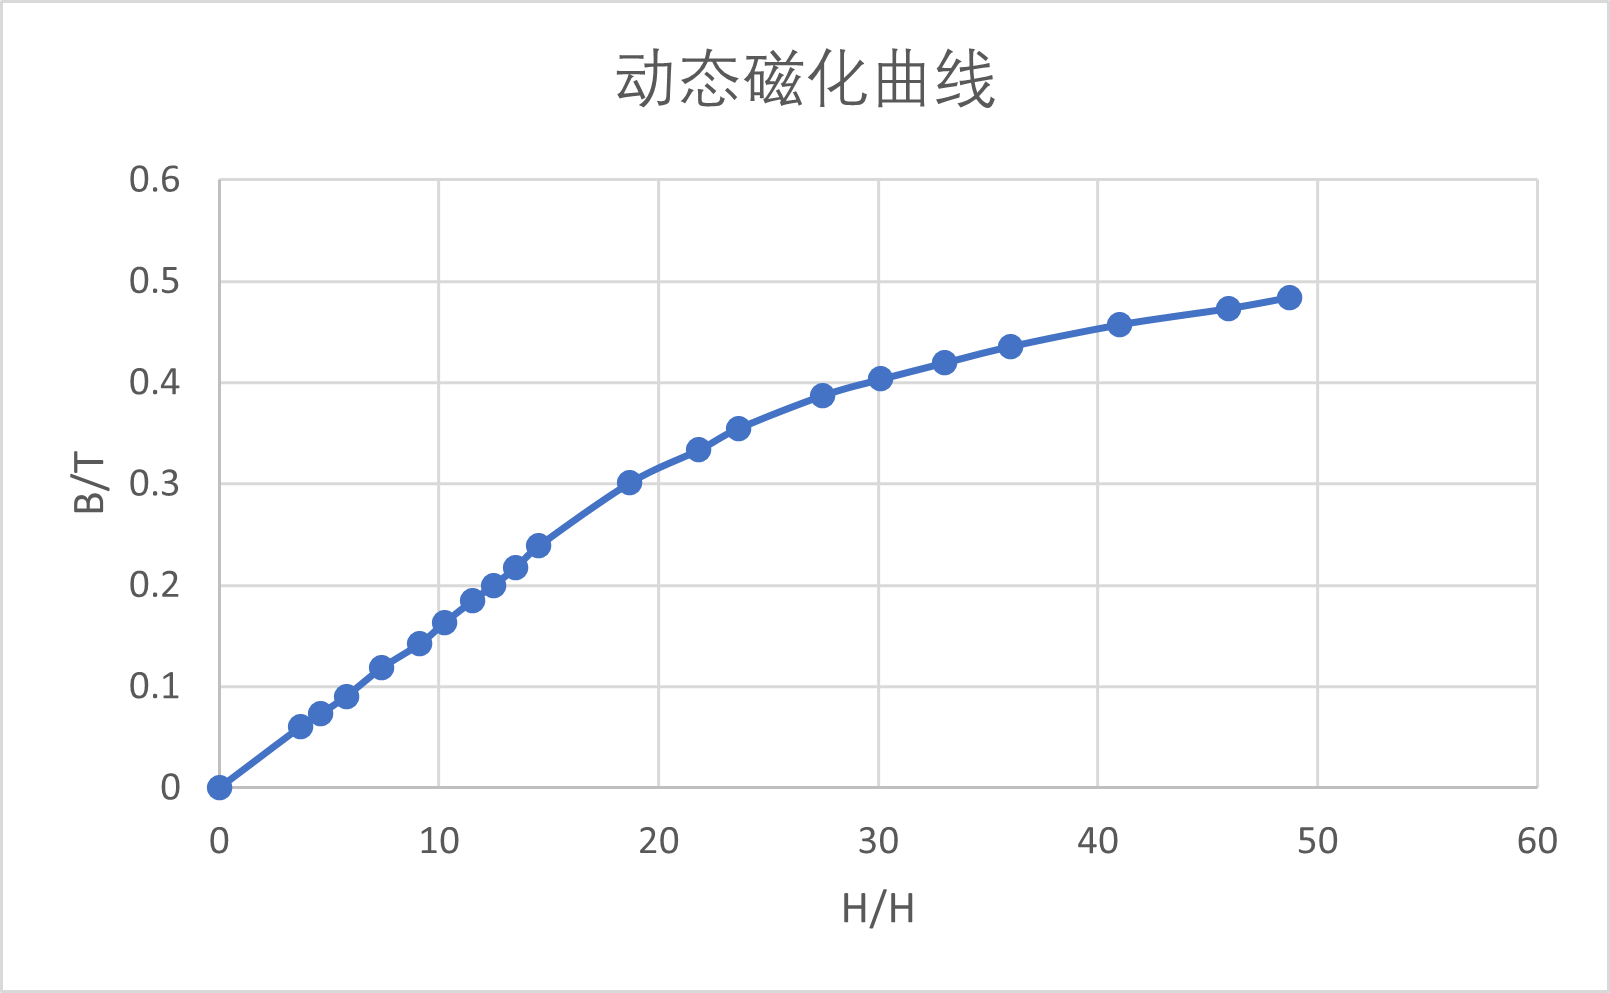
\includegraphics[width=8cm]{Fig/6.png}
                \caption{动态磁化曲线}
            \end{minipage}
            \begin{minipage}[t]{0.49\linewidth}
                \centering
                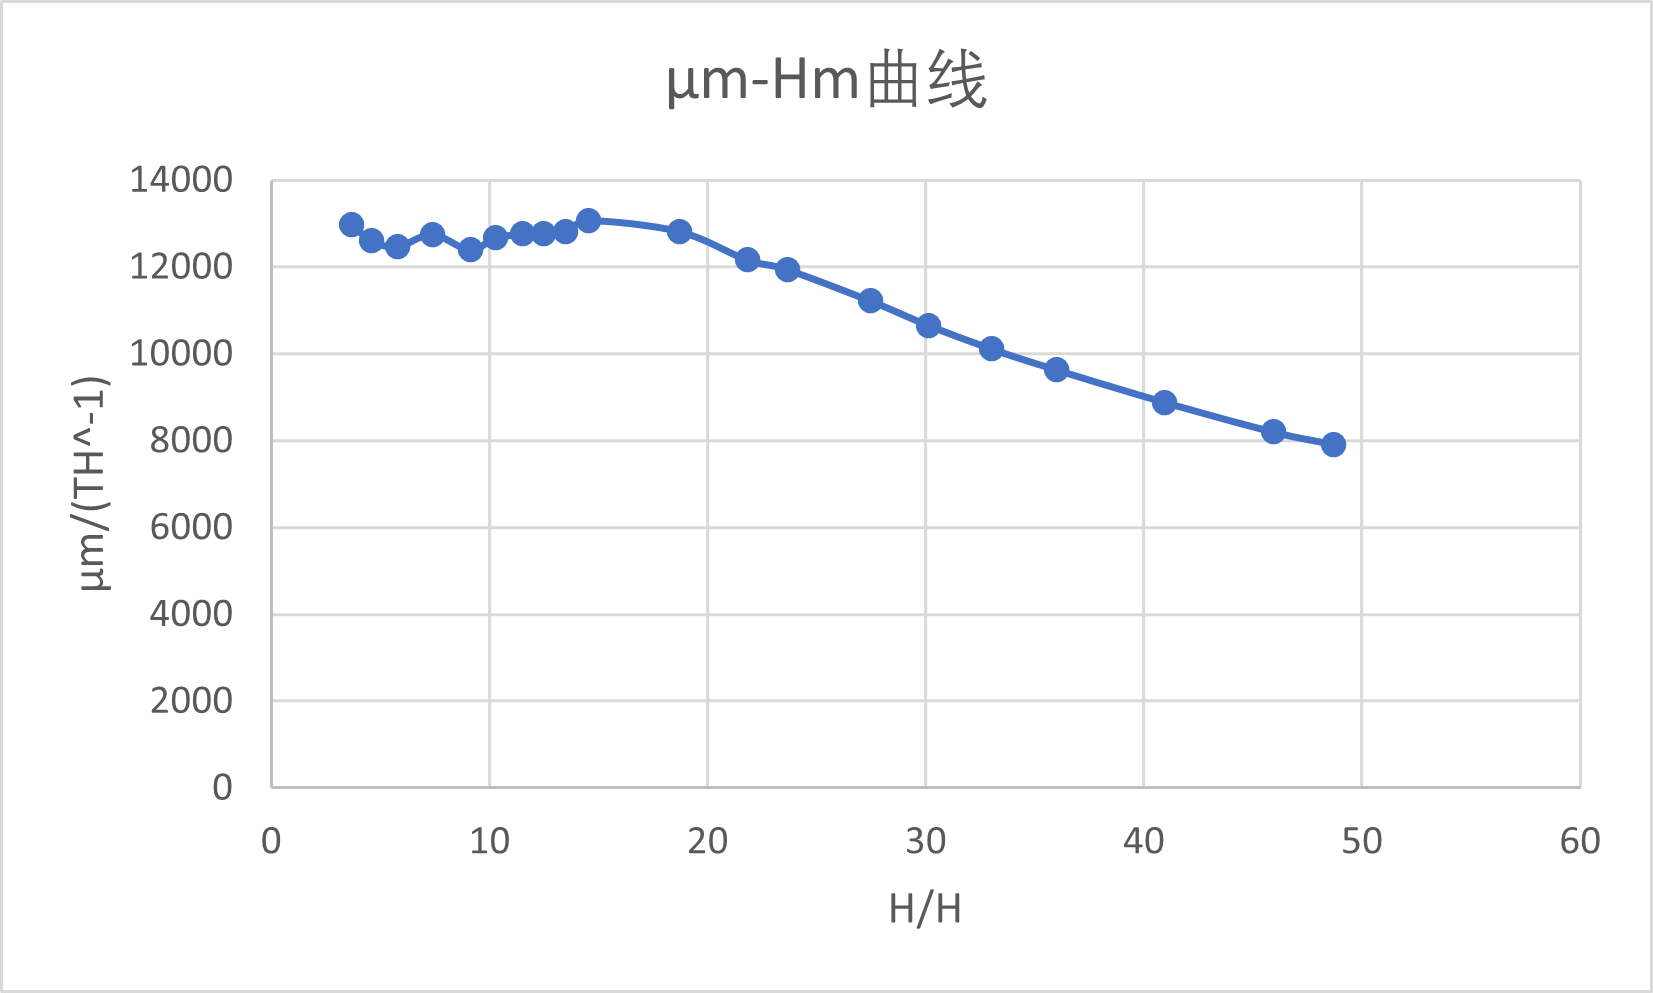
\includegraphics[width=8cm]{Fig/7.png}
                \caption{$\mu_m - H_m$曲线}
            \end{minipage}
            
        \end{figure}
        
        \hspace*{2em}可以看到,动态磁化曲线和预期相符,$\mu_m - H_m$曲线与预期有差别。可能的原因是:我们可以认为测量误差是恒定的零点几毫伏,振幅较小时,误差对$\mu_m$的影响较大,体现在图像中动态磁化曲线误差不大但是$\mu_m - H_m$误差大。同时我测量的$H_m$的范围较小,前期点过密,导致图像不理想。
        \newline \hspace*{2em} 同时这也可能是由于铁磁性物质温度升高导致磁导率下降,在测量时样品温度升高,后续磁导率相较于初始状态偏低导致的。

\end{enumerate}
\subsection{观察不同频率下样品2(硅钢)的动态磁滞回线}
\begin{enumerate}
    \item 调整设备,使$R_1=2.0\Omega$, $R_2=50k\Omega$, $C=10.0\mu F$。
    \item 改变频率,测量$B_m$,$B_r$,$H_c$。
    \item 实验中测量$H$与$B$是按电压$u/mV$记录的。根据$H=\frac{N_1}{lR_1}u_{R_1}=1000u_{R_1}$,$B=\frac{R_2C}{N_2S}u_C=27.8u_C$修正实验数据。
            % Table generated by Excel2LaTeX from sheet 'Sheet1'
        \begin{table}[H]
          \centering
          \caption{样品2动态磁化曲线数值}
            \begin{tabular}{|c|c|c|c|}\hline
            $f/Hz$    & 20   & 40   & 60 \\\hline
            $u_{B_m}/mV$   & 32.8   & 32.8   & 32.8 \\\hline
            $u_{B_r}/mV$   & 19.6   & 21.2   & 22.2 \\\hline
            $u_{H_c}/mV$   & 96     & 114    & 133 \\\hline
            $B_m/T$  & 0.9118  & 0.9118  & 0.9118  \\\hline
            $B_r/T$  & 0.5449  & 0.5894  & 0.6172  \\\hline
            $H_c/H$  & 96     & 114    & 133 \\\hline
            \end{tabular}%
          \label{tab:动态磁化2}%
        \end{table}%
    可以看到,$B_m$不随频率变化而变化,$B_r$和$H_c$随频率增大而增大。
\end{enumerate}
\subsection{测量样品1(铁氧体)在不同直流偏置磁场下的可逆磁导率}
\begin{enumerate}
    \item 调整设备,使$f=100Hz$, $R_1=2.0\Omega$, $R_2=20k\Omega$, $C=2.0\mu F$。
    \item 直流偏置磁场从0到$H_s$单调增加。调整输出振幅,保证磁滞回线为近似线性,此段磁导率为可逆磁导率。测量十组回线小线段的$B_m=\Delta B$与$H_m=\Delta H$与。
    \item 实验中测量$H$与$B$是按电压$u/mV$记录的。根据$H=\frac{N_1}{lR_1}u_{R_1}=577u_{R_1}$,$B=\frac{R_2C}{N_2S}u_C=2.15u_C$修正实验数据。
    \item $\mu_i=\lim\limits_{H\to 0} \frac{B}{\mu_0 H} $。测量中保证$\Delta H$很小,近似认为$\mu_i=\frac{\Delta B}{\mu_0 \Delta H} $。
    \item 由$H_r=I\frac{N_3}{l}=1154I$计算之。
    \item 实验数据
            % Table generated by Excel2LaTeX from sheet 'Sheet1'
        \begin{table}[H]
          \centering
          \caption{不同直流偏置磁场下的可逆磁导率}
            \begin{tabular}{|c|c|c|c|c|c|c|}\hline
            $I/A$    & 端点坐标$H1/mV$     & 端点坐标$B1/mV$     & $\Delta H/H$      & $\Delta B/T$      & $\mu_i /(T\cdot H^{-1})$     & $H_r/H$ \\\hline
            0.01   & 6.08   & 14.2   & 3.508  & 0.03053 & 6925.29  & 11.54 \\\hline
            0.02   & 9.36   & 14.4   & 5.401  & 0.03096 & 4561.84  & 23.08 \\\hline
            0.03   & 15.4   & 15     & 8.886  & 0.03225 & 2888.18  & 34.62 \\\hline
            0.04   & 9.2    & 5.2    & 5.308  & 0.01118 & 1675.98  & 46.16 \\\hline
            0.05   & 10.4   & 4.08   & 6.001  & 0.008772 & 1163.27  & 57.7 \\\hline
            0.06   & 12.4   & 3.44   & 7.155  & 0.007396 & 822.60  & 69.24 \\\hline
            0.07   & 18.2   & 3.76   & 10.501  & 0.008084 & 612.59  & 80.78 \\\hline
            0.08   & 12.6   & 2.16   & 7.270  & 0.004644 & 508.32  & 92.32 \\\hline
            0.09   & 12.6   & 1.76   & 7.270  & 0.003784 & 414.19  & 103.86 \\\hline
            0.1    & 12     & 1.44   & 6.924  & 0.003096 & 355.82  & 115.4 \\\hline
            \end{tabular}%
          \label{tab:可逆磁导率}%
        \end{table}%
        \begin{figure}[H]
            \centering
            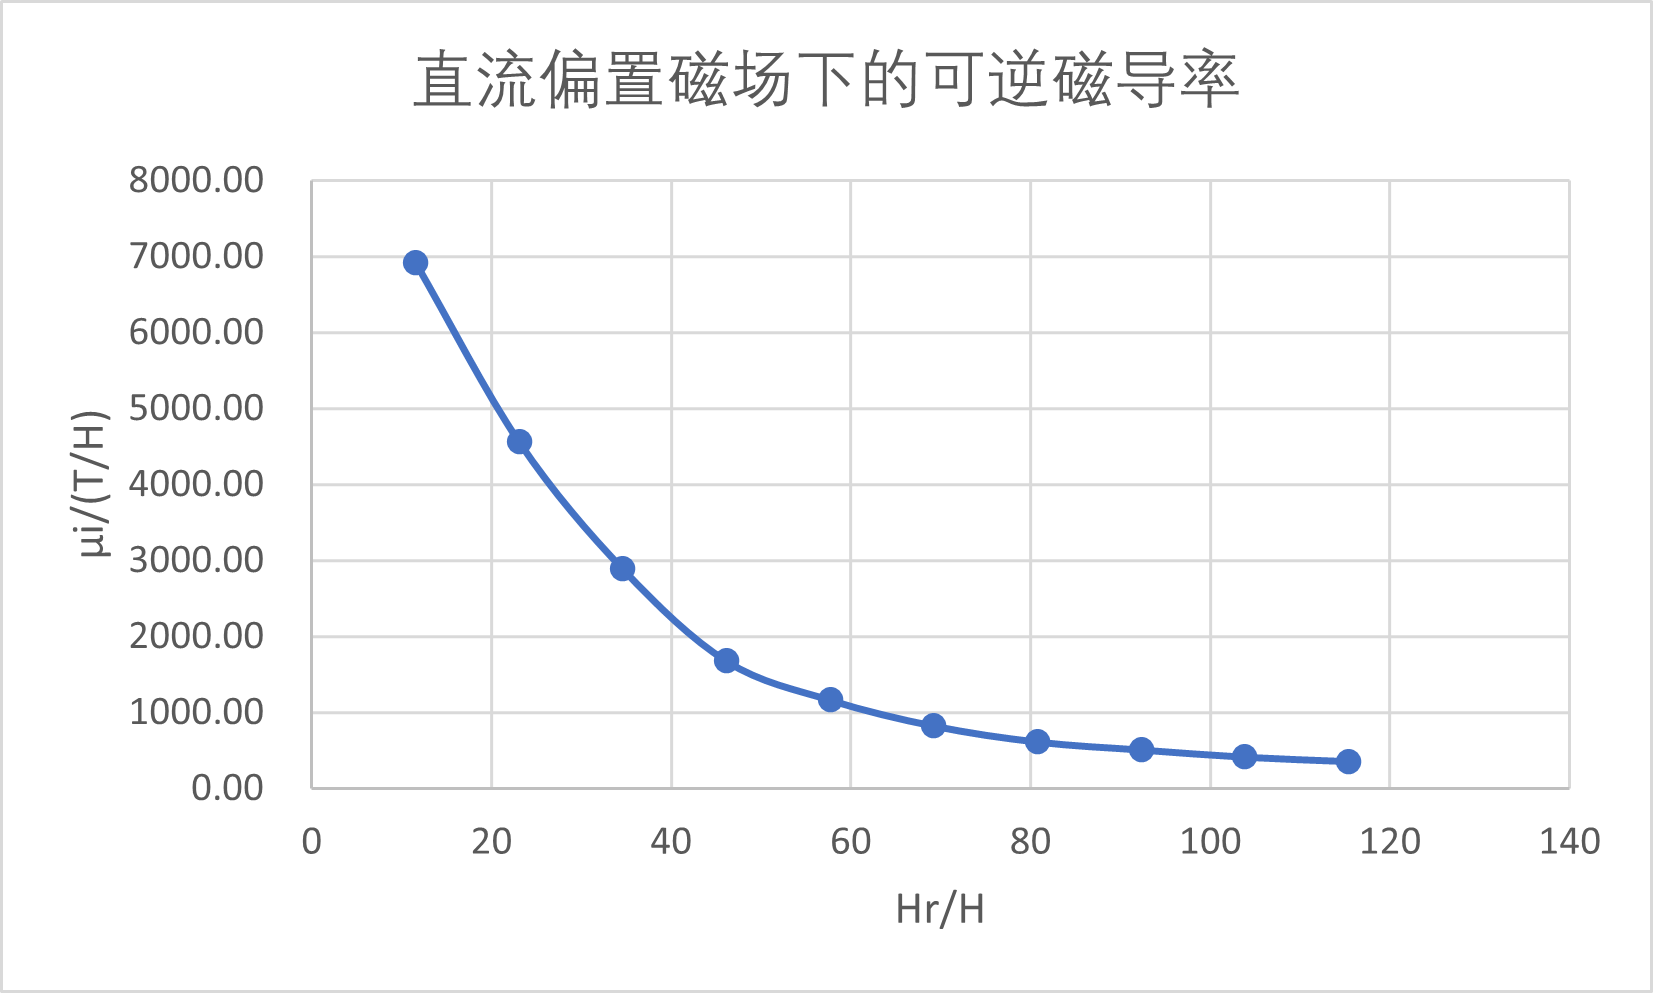
\includegraphics[width=9cm]{Fig/8.png}
            \caption{可逆磁导率随外场强度的变化曲线}
        \end{figure}
        \hspace*{2em} 查询资料得,铁氧体可逆磁导率$\mu_i$范围在$10^3\sim 10^4$,测量结果合理。
        \newline \hspace*{2em}可以看到,随着直流偏置磁场强度上升,可逆磁导率下降。直流偏置磁场强度较小时,可逆磁导率下降较快。直流偏置磁场强度足够大时,可逆磁导率趋近于0,说明磁滞回线线性区域长度趋于0。

\end{enumerate}
\section{用霍尔传感器测量铁磁材料(准)静态磁滞回线}
\subsection{测量样品的起始磁化曲线}
\begin{enumerate}
    \item 将霍尔传感器置于磁场均匀区的中央。反复进行退磁操作,使电流为0时磁感应强度在$\pm 0.5mT$范围内。(实际实验时为$-0.1mT$)
    \item 电流从$0mA$到$600mA$取20个采样点,测量磁感应强度$B$并记录。
    \item $H=\frac{N}{\tilde{l}}I=8333I$,$H_{\text{修正}}=\frac{1}{\tilde{l}} \left(NI-\frac{1}{\mu_0}Bl_g\right)=8333I-6631B$分别计算$H$和$H_{\text{修正}}$。
    \item 实验数据
    % Table generated by Excel2LaTeX from sheet 'Sheet1'
        \begin{table}[H]
          \centering
          \caption{模具钢起始磁化曲线数据}
            \begin{tabular}{|c|c|c|c|c|c|c|c|}\hline
            $I/mA$ & $B/mT$ & $H/H$ & $H_{\text{修正}}/H$ & $I/mA$ & $B/mT$ & $H/H$ & $H_{\text{修正}}/H$ \\\hline
            0      & -0.1   & 0.00   & 0.66   & 330.1  & 152.2  & 2750.72  & 1741.49  \\\hline
            30.2   & 4.3    & 251.66  & 223.14  & 360.3  & 171.7  & 3002.38  & 1863.84  \\\hline
            60     & 10.8   & 499.98  & 428.37  & 389.8  & 190.3  & 3248.20  & 1986.32  \\\hline
            90.2   & 17.8   & 751.64  & 633.60  & 420.1  & 208.9  & 3500.69  & 2115.48  \\\hline
            120.1  & 28.3   & 1000.79  & 813.14  & 450.3  & 227.4  & 3752.35  & 2244.46  \\\hline
            150.4  & 43.8   & 1253.28  & 962.85  & 480.1  & 245.5  & 4000.67  & 2372.76  \\\hline
            180.1  & 59.9   & 1500.77  & 1103.58  & 509.9  & 263.2  & 4249.00  & 2503.72  \\\hline
            210.3  & 75.6   & 1752.43  & 1251.13  & 540.2  & 279.8  & 4501.49  & 2646.13  \\\hline
            240.5  & 92.8   & 2004.09  & 1388.73  & 570    & 295.6  & 4749.81  & 2789.69  \\\hline
            270.2  & 112.4  & 2251.58  & 1506.25  & 600.1  & 310.1  & 5000.63  & 2944.36  \\\hline
            300    & 132.2  & 2499.90  & 1623.28  &        &        &        &  \\\hline

            \end{tabular}%
          \label{tab:模具钢起始磁化曲线}%
        \end{table}%
        \begin{figure}[H]
            \centering
            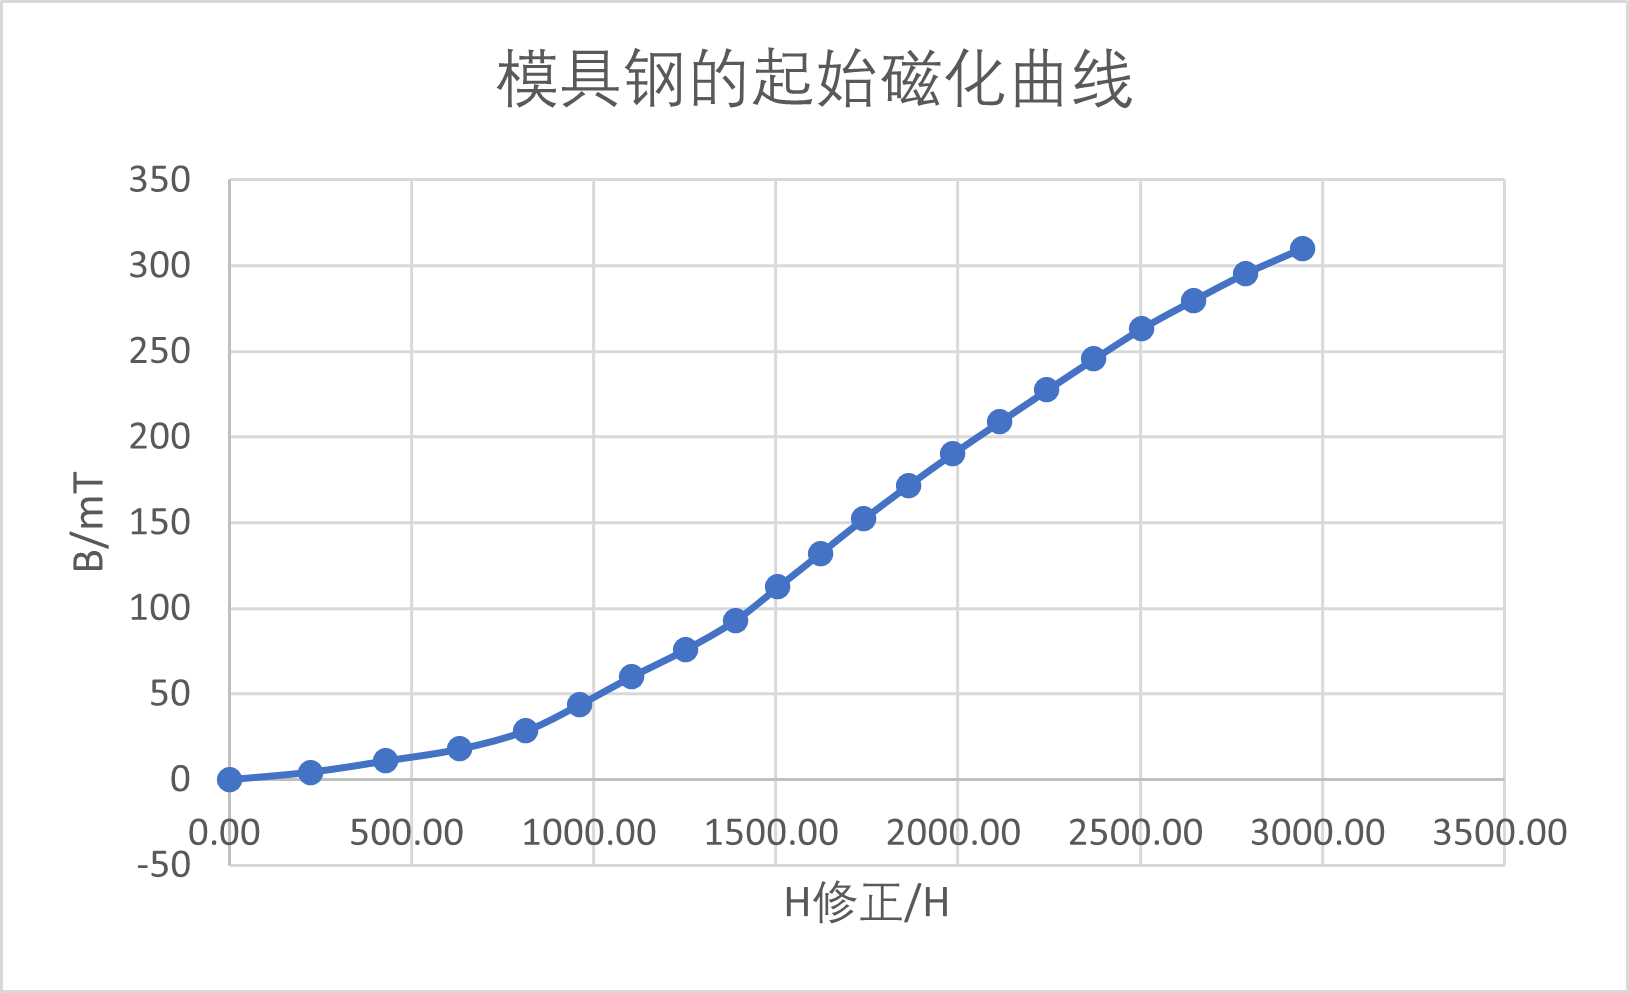
\includegraphics[width=9cm]{Fig/9.png}
            \caption{模具钢起始磁化曲线}
        \end{figure}


\end{enumerate}
\subsection{测量模具钢的磁滞回线}
\begin{enumerate}
    \item 反复按电流方向开关8-10次进行磁锻炼
    \item 调整电流,每隔$50mA$测一组(I,B),并记录。
    \item $H=\frac{N}{\tilde{l}}I=8333I$,$H_{\text{修正}}=\frac{1}{\tilde{l}} \left(NI-\frac{1}{\mu_0}Bl_g\right)=8333I-6631B$分别计算$H$和$H_{\text{修正}}$。
    \item 实验数据
    \begin{figure}[H]
        \centering
        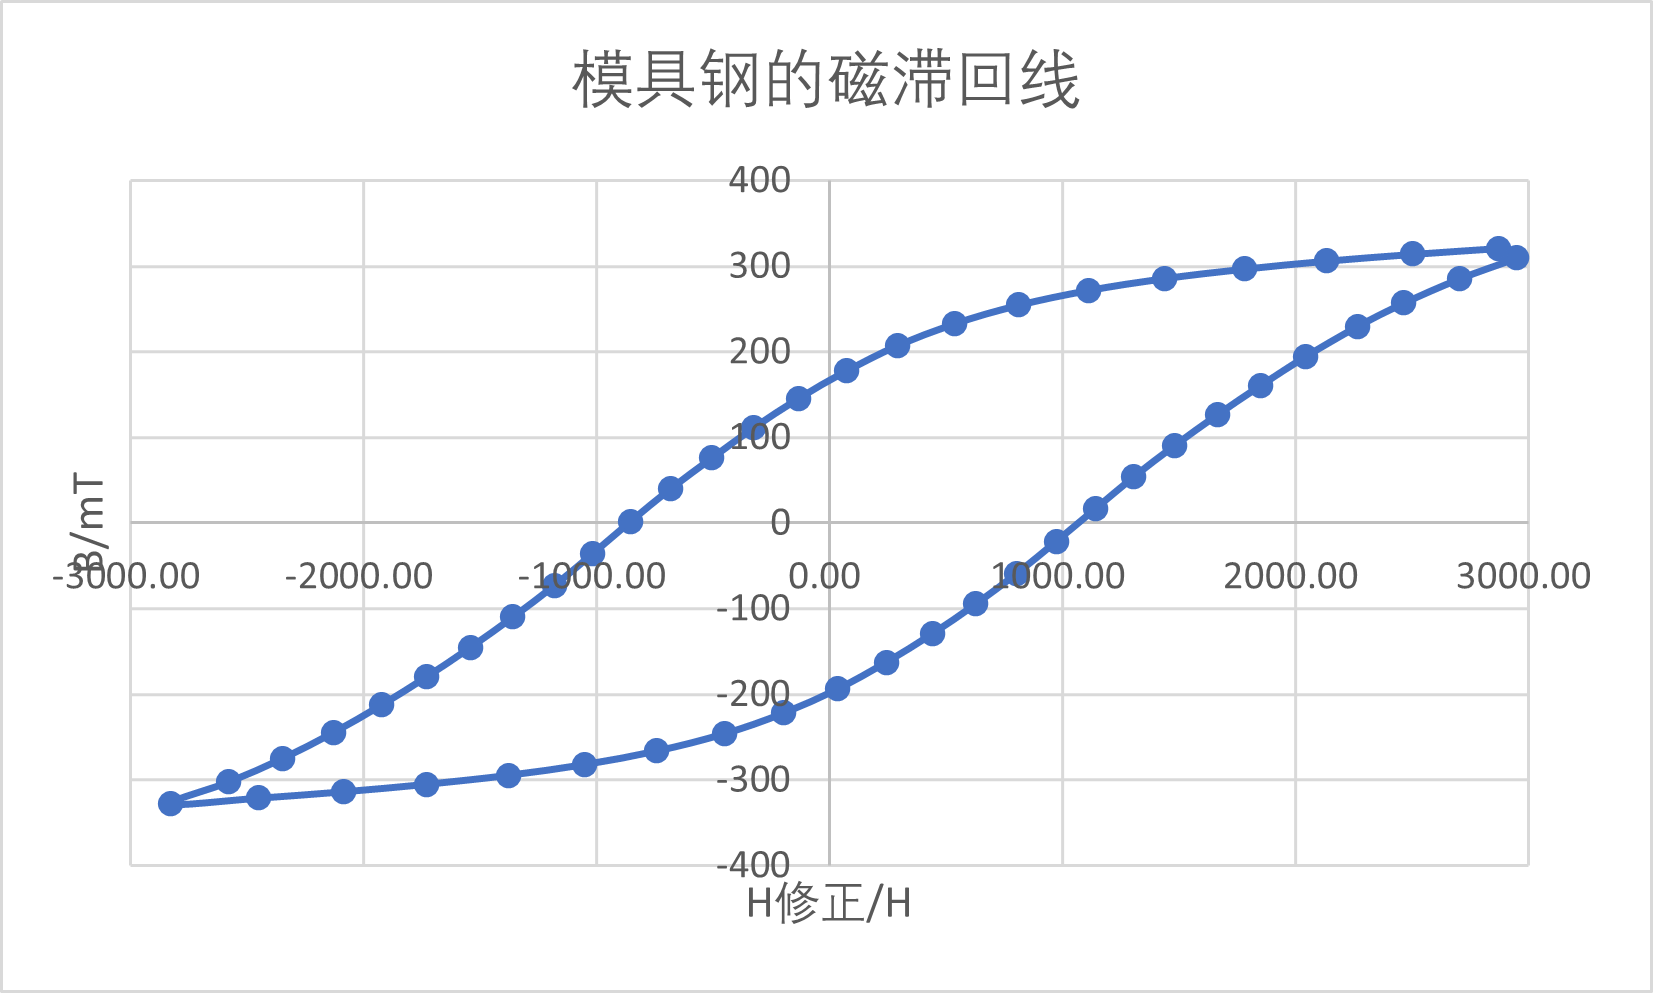
\includegraphics[width=9cm]{Fig/10.png}
        \caption{模具钢的磁滞回线}
    \end{figure}
    \hspace*{2em}磁滞回线基本闭合。磁滞回线右上角未完全闭合,有很小的差别。这可能是过程中样品温度变化导致的。畴壁可以通过热起伏向能量更小的位置移动,导致系统的自由能变小。
    % Table generated by Excel2LaTeX from sheet 'Sheet1'
        \begin{table}[H]
          \centering
          \caption{模具钢的磁滞回线数据}
            \begin{tabular}{|c|c|c|c|c|c|c|c|}\hline
            I      & B      & H      & H修正    & I      & B      & H      & H修正 \\\hline
            600.2  & 321    & 5001.47  & 2872.92  & -549.7 & -321   & -4580.65  & -2452.10  \\\hline
            550.3  & 314.2  & 4585.65  & 2502.19  & -499.8 & -313.5 & -4164.83  & -2086.01  \\\hline
            499.6  & 306.2  & 4163.17  & 2132.75  & -450.2 & -304.8 & -3751.52  & -1730.39  \\\hline
            450.2  & 297    & 3751.52  & 1782.11  & -399.7 & -294.3 & -3330.70  & -1379.20  \\\hline
            400.1  & 285.9  & 3334.03  & 1438.23  & -350.1 & -281.7 & -2917.38  & -1049.43  \\\hline
            349.9  & 272    & 2915.72  & 1112.08  & -300.3 & -265.8 & -2502.40  & -739.88  \\\hline
            299.9  & 254.6  & 2499.07  & 810.81  & -249.7 & -245.8 & -2080.75  & -450.85  \\\hline
            250.2  & 233.2  & 2084.92  & 538.57  & -200.2 & -221.8 & -1668.27  & -197.51  \\\hline
            200    & 207.3  & 1666.60  & 291.99  & -149.6 & -193.4 & -1246.62  & 35.82  \\\hline
            150.3  & 177.9  & 1252.45  & 72.80  & -99.9  & -162.4 & -832.47  & 244.41  \\\hline
            99.9   & 145.6  & 832.47  & -133.01  & -50    & -129.3 & -416.65  & 440.74  \\\hline
            49.6   & 111.4  & 413.32  & -325.38  & 0      & -94.6  & 0.00   & 627.29  \\\hline
            0      & 76.1   & 0.00   & -504.62  & 50     & -58.6  & 416.65  & 805.23  \\\hline
            -50.1  & 40     & -417.48  & -682.72  & 99.9   & -21.3  & 832.47  & 973.71  \\\hline
            -100.5 & 2.3    & -837.47  & -852.72  & 150    & 16.5   & 1249.95  & 1140.54  \\\hline
            -150.3 & -35.6  & -1252.45  & -1016.39  & 200.1  & 54.3   & 1667.43  & 1307.37  \\\hline
            -199.9 & -73    & -1665.77  & -1181.70  & 249.9  & 90.6   & 2082.42  & 1481.65  \\\hline
            -250.1 & -109.5 & -2084.08  & -1357.99  & 300.5  & 126.5  & 2504.07  & 1665.25  \\\hline
            -300.3 & -145   & -2502.40  & -1540.90  & 350    & 160.7  & 2916.55  & 1850.95  \\\hline
            -350   & -179.2 & -2916.55  & -1728.27  & 400.1  & 194.5  & 3334.03  & 2044.30  \\\hline
            -400   & -212.5 & -3333.20  & -1924.11  & 454.5  & 229.5  & 3787.35  & 2265.53  \\\hline
            -450.1 & -244.5 & -3750.68  & -2129.40  & 500.3  & 256.9  & 4169.00  & 2465.50  \\\hline
            -499.9 & -274.5 & -4165.67  & -2345.46  & 551.8  & 285.4  & 4598.15  & 2705.66  \\\hline
            -549.9 & -302.2 & -4582.32  & -2578.43  & 600.6  & 309.6  & 5004.80  & 2951.84  \\\hline
            -600.1 & -327.7 & -5000.63  & -2827.65  &        &        &        &  \\\hline
            \end{tabular}%
          \label{tab:addlabel}%
        \end{table}%

\end{enumerate}
\section{实验反思、收获与总结}
\subsection{思考题}
\begin{enumerate}
    \item 铁磁材料的动态磁滞回线与(准)静态磁滞回线在概念上有什么区别?铁磁材料动态
    磁滞回线的形状和面积受那些因素影响?
    \newline 区别:
    \newline \hspace*{2em}铁磁材料的动态磁滞回线是在交变电场的作用下,得到的 B-H关系曲线,而静
    态磁滞回线 仅记录了直流电场作用下磁化完全后的 B-H关系曲线。
    \newline \hspace*{2em}影响因素:两种磁滞回线都受到铁磁材料种类、大小影响。动态磁滞回线还受到交流电频率,磁化场的大小等多种因素的影
    响,其围成的面积等于一个周期的能量损耗,这些损耗除了磁滞损耗外,还包括涡流损耗与
    剩余损耗。静态磁滞回线仅受到磁化场的大小影响,因为没有磁场大小随时间的变化,因此几乎没有涡流损耗和剩余损耗。
    \newline \hspace*{2em}在低频磁场下,动态磁滞回线与静态磁滞回线类似,表现出明显的剪切滞后效应。但在高频磁场下,动态磁滞回线会出现一系列特征,如剪切滞后减小、磁滞损耗增加、饱和磁化强度降低等。本实验为低频磁场,因此动态磁滞回线与静态磁滞回线类似。
    \item 什么叫做基本磁化曲线?它和起始磁化曲线间有何区别?
    \newline \hspace*{2em}起始磁化曲线是将一块从未磁化过(或退磁后)的铁磁材料放入磁场中进行磁化,所得的B-H曲线。测量时,B和H从0开始单调上升;
    基本磁化曲线是对同一铁磁材料,选择不同的磁场强度进行反复磁化,可得一系列大小不同的磁滞回线,再将各磁滞回线的顶点连接所得的曲线。
    \item 铁氧体和硅钢材料的动态磁化特性各有什么特点?
    \newline \hspace*{2em} 首先,铁氧体的高频特性非常好,因为其磁滞损耗很小,矫顽力也低。其次,铁氧体的低温系数也比一般的合金低,因此在低温环境下也能够保持稳定的性能。此外,铁氧体的能耗非常小,因为它的磁导率很高,这也是它成为高频器件的主要原因。但是铁氧体饱和磁感应强度较低。
    \newline \hspace*{2em}硅钢材料是一种低碳高硅的冷轧电工钢板材,具有低频饱和磁感应强度高等优点。硅钢的低频饱和磁感应强度一般能达到2T以上,因此在一些低频大电流的应用中得到了广泛的应用。此外,硅钢的磁滞损耗也比较小,其矫顽力也比较低,因此在高磁通密度下可以保持较高的磁导率,常用于变压器中。
        虽然硅钢的饱和磁感应强度高,但其高频特性与铁氧体相比会有所逊色,因此在高频应用中不太合适。
    \newline \hspace*{2em}在实际使用时,应选择合适的材料,以满足不同的应用需求。
    \item 动态磁滞回线测量实验中,电路参量应怎样设置才能保证$u_{R1}-u_C$所形成的李萨如图形正确反映材料动态磁滞回线的形状?
    \newline \hspace*{2em} 在计算交流磁感应强度时,在公式推导中要求时间常数$R_2C\gg T$,T为外电场周期。此时保证了电容C上的电压远远小于$U_{2}$,电阻$R_2$上的电压$U_{R2}$近似等于$U_{2}$。
    \newline \hspace*{2em} 为了减小交流磁场在线圈3 中产生的感应信号对直流稳定性的影响,需要在回路中串入一只大电感L。
    \newline \hspace*{2em} 在实际科研测量时,应使待测样品满足$H\tilde{l}\gg \frac{1}{\mu_0}Bl_g$,即平均磁路总长度$\tilde{l}$足够大,间隙$l_g$尽可能小。这时$H\tilde{l}\gg\approx NI$,可以不进行$H$计算的修正。在示波器显示图像时,这很重要。但在后期处理数据时,可进行$H$计算的修正,此项影响可忽略。
    \item 准静态磁滞回线测量实验中,为什么要对样品进行磁锻炼才能获得稳定的饱和磁滞回线?
    \begin{figure}[H]
        \centering
        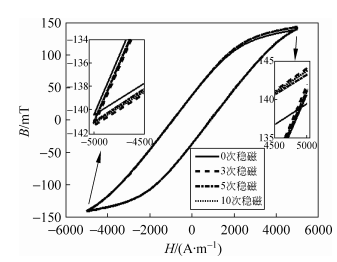
\includegraphics[width=8cm]{Fig/11.png}
        \caption{磁锻炼次数不同时Cr12模具钢的磁滞回线,来源于网络}
    \end{figure}
    \hspace*{2em} 磁锻炼是一种稳磁的方法。为了使磁铁的性能更稳定,从而得到稳定闭合的磁滞回线。在实际操作中,多次开关换向开关会造成损耗。如图10,磁锻炼5次-10次即可达到目的,本实验也大致磁锻炼此次数。
    \newline \hspace*{2em}磁锻炼过程的原理,是使剩磁对正反向磁化的作用效果相等,或者说在描绘磁滞回线时,使正反向剩磁的大小相等,从而使磁滞回线闭合。并不是由于磁锻炼造成升温减小阻力使磁滞回线闭合。

\end{enumerate}
\subsection{反思与总结}
\begin{enumerate}
    \item 在动态磁滞回线实验部分,应调整示波器振幅与相位到合适位置,以提高测量精度。如测量某个特定点时,可减小振幅放大图像。
    \item 在我的实验中,$H_c$的测量应该存在错误,特别是频率增高时$H_c$应减小而不是不变。可能是在双光标的情况下,我读数读成了未移动的光标的值,导致测量错误。
    \item 铁磁质磁导率随温度变化明显,因此本实验中样品温度变化对实验结果影响很大,应速战速决。
    \item $\mu_m - H_m$图像与理想中严重不符合,在$H_m$较小时$\mu_m$应随$H_m$增大而增大,但测量结果是持平。主要原因可能是振幅较小时,我的读数误差较大导致的。次要原因是前期$H_c$测量错误导致了测量范围选取错误,测量点间距不佳。
    \item 模具钢的起始磁化曲线和磁滞回线测量结果较好,原因是退磁比较成功,以及磁锻炼比较成功。实际操作中,慢一点拧动电流旋钮,会使实验结果更理想。
    \item 本实验动态磁滞回线部分测量量全部为电压振幅,需要依照公式转换为磁场强度和磁感应强度,要注意不同实验的参数不同导致转换比例不同。
    \item 总结地来讲,有关示波器的读数均需要仔细,因为图像很可能不是稳定的。对于关键点的测量,未来可以多次测量防止测量错误带来的影响。多组数据测量时要选取合适的测量范围和测量间隔,以得出效果更好的图像。选取测量间隔过小再加上测量误差的不稳定,会使图像光滑性降低。
\end{enumerate}

\begin{center}
    \vspace*{1em}
    \Large \bf 第二部分\qquad 实验原始记录
\end{center}
\includepdf[pages={1-4}]{Data/磁滞回线实验报告.pdf}

\end{document}